%%%%%%%%%%%%%%%%%%%%%%%%%%%%%%%%%%%%%%%%%%%%%%%%%%%%%%%%%%%%%%%%%%%%%%%%%%%%%%%%
%% Plantilla de memoria en LaTeX para la EIF - Universidad Rey Juan Carlos
%%
%% Por Gregorio Robles <grex arroba gsyc.urjc.es>
%%     Grupo de Sistemas y Comunicaciones
%%     Escuela de Ingeniería de Fuenlabrada
%%     Universidad Rey Juan Carlos
%% (muchas ideas tomadas de Internet, colegas del GSyC, antiguos alumnos...
%%  etc. Muchas gracias a todos)
%%
%% La última versión de esta plantilla está siempre disponible en:
%%     https://github.com/gregoriorobles/plantilla-memoria
%%
%% Para obtener PDF, ejecuta en la shell:
%%   make
%% (las imágenes deben ir en PNG o JPG)

%%%%%%%%%%%%%%%%%%%%%%%%%%%%%%%%%%%%%%%%%%%%%%%%%%%%%%%%%%%%%%%%%%%%%%%%%%%%%%%%

\documentclass[a4paper, 12pt]{book}
%\usepackage[T1]{fontenc}

\usepackage[a4paper, left=2.5cm, right=2.5cm, top=3cm, bottom=3cm]{geometry}
\usepackage{times}
\usepackage[utf8]{inputenc}
\usepackage[spanish]{babel} % Comenta esta línea si tu memoria es en inglés
\usepackage{url}
%\usepackage[dvipdfm]{graphicx}
\usepackage{graphicx}
\usepackage{float}  %% H para posicionar figuras
\usepackage[nottoc, notlot, notlof, notindex]{tocbibind} %% Opciones de índice
\usepackage{latexsym}  %% Logo LaTeX
\usepackage{tikz}
\usepackage{array}

% Escribe el título y el nombre del autor / autora para que se use bien
% en otras partes de la plantilla
% Dependiendo de las partes de la plantilla, a veces aparecerán tal
% cual los escribas, a veces totalmente en mayúsculas, a veces de otras
% formas
\title{Rediseño de aplicación de análisis de código Python}
\author{ José Matas Luque}

% Guarda el título, el autor y la fecha en variables
\makeatletter
\let\thetitle\@title
\let\theauthor\@author
\let\thedate\@date
\makeatother

\renewcommand{\baselinestretch}{1.5}  %% Interlineado

\begin{document}

\renewcommand{\refname}{Bibliografía}  %% Renombrando
\renewcommand{\appendixname}{Apéndice}


%%%%%%%%%%%%%%%%%%%%%%%%%%%%%%%%%%%%%%%%%%%%%%%%%%%%%%%%%%%%%%%%%%%%%%%%%%%%%%%%
% PORTADA

\begin{titlepage}
\begin{center}
\includegraphics[scale=0.6]{img/URJ_logo_Color_POS.png}

\vspace{1.75cm}

\LARGE
ESCUELA DE INGENIERÍA DE FUENLABRADA
\vspace{1cm}

\LARGE
Ingeniería en Tecnologías de la Telecomunicación

\vspace{1cm}
\LARGE
\textbf{TRABAJO FIN DE GRADO}

\vspace{2cm}

\Large
\MakeUppercase{\thetitle}

\vspace{2cm}

\large
Autor : \theauthor \\
Tutor : Dr. Gregorio Robles Martínez\\
\vspace{1cm}

\large
Curso académico 2024/2025

\end{center}
\end{titlepage}

\newpage
\mbox{}
\thispagestyle{empty} % para que no se numere esta pagina



%%%%%%%%%%%%%%%%%%%%%%%%%%%%%%%%%%%%%%%%%%%%%%%%%%%%%%%%%%%%%%%%%%%%%%%%%%%%%%%%
%%%% Para firmar
\clearpage
\pagenumbering{gobble}
\chapter*{}

\vspace{-4cm}
\begin{center}
\LARGE
\textbf{Trabajo Fin de Grado}

\vspace{1cm}
\large
\thetitle

\vspace{0.8cm}
\large
\textbf{Autor :} \theauthor \\
\textbf{Tutor :} Dr. Gregorio Robles Martínez

\end{center}

\vspace{0.8cm}
La defensa del presente Proyecto Fin de Carrera se realizó el día \qquad$\;\,$ de \qquad\qquad\qquad\qquad \newline de 2024, siendo calificada por el siguiente tribunal:


\vspace{0.5cm}
\textbf{Presidente:}

\vspace{1cm}
\textbf{Secretario:}

\vspace{1cm}
\textbf{Vocal:}


\vspace{1cm}
y habiendo obtenido la siguiente \textbf{Calificación:}


\vspace{1cm}
\begin{flushright}
Fuenlabrada, a \qquad$\;\,$ de \qquad\qquad\qquad\qquad de 202X
\end{flushright}

\vspace{1cm}

%% Licencia de publicación en abierto elegida
%% Ver detalles en https://ofilibre.urjc.es/guias/tfg-abierto/
\includegraphics[scale=0.6]{img/by-sa}
%\includegraphics[scale=0.6]{img/by}

%% Poner el año adecuado
\noindent©2024 \theauthor  \\
Algunos derechos reservados  \\
Este documento se distribuye bajo la licencia ``Atribución-CompartirIgual 4.0 Internacional'' de Creative Commons, disponible en \\
\url{https://creativecommons.org/licenses/by-sa/4.0/deed.es}


%%%%%%%%%%%%%%%%%%%%%%%%%%%%%%%%%%%%%%%%%%%%%%%%%%%%%%%%%%%%%%%%%%%%%%%%%%%%%%%%
%%%% Dedicatoria

\pagenumbering{Roman} % para comenzar la numeracion de paginas en numeros romanos
%\begin{flushright}
%\textit{Dedicado a \\
%mi familia / mi abuelo / mi abuela}
%\end{flushright}

%%%%%%%%%%%%%%%%%%%%%%%%%%%%%%%%%%%%%%%%%%%%%%%%%%%%%%%%%%%%%%%%%%%%%%%%%%%%%%%%
%%%% Agradecimientos

\chapter*{Agradecimientos}
%\addcontentsline{toc}{chapter}{Agradecimientos} % si queremos que aparezca en el índice
\markboth{AGRADECIMIENTOS}{AGRADECIMIENTOS} % encabezado 

Quisiera expresar mi más sincero agradecimiento a todas aquellas personas que, de una forma u otra, me han acompañado durante estos años, siendo parte de este largo camino cuyo fin llega con la realización de este proyecto.

En primer lugar, quiero agradecer profundamente a mi familia, cuyo amor y apoyo me han otorgado el ánimo y confianza necesarios en esta etapa.

A mis amigos y compañeros, quienes han vivido conmigo este viaje académico, gracias por los momentos compartidos y por todo lo que me han permitido aprender.

Por último, quisiera agradecer también a los profesores que han contribuido a mi formación durante este ciclo, permitiéndome llegar hasta aquí. En particular un especial agradecimiento a mi tutor, Gregorio Robles, por la paciencia y la ayuda dada durante el desarrollo de este proyecto.
%%%%%%%%%%%%%%%%%%%%%%%%%%%%%%%%%%%%%%%%%%%%%%%%%%%%%%%%%%%%%%%%%%%%%%%%%%%%%%%%
%%%% Resumen

\chapter*{Resumen}
%\addcontentsline{toc}{chapter}{Resumen} % si queremos que aparezca en el índice
\markboth{RESUMEN}{RESUMEN} % encabezado

El objetivo principal de este proyecto es rediseñar y extender la funcionalidad de la ya existente aplicación ``pycefrl'', con el fin de hacerla más accesible y cómoda de usar e interpretar para el usuario. Esta herramienta tiene como labor realizar análisis de código en el lenguaje Python para obtener un nivel de complejidad ajustado a los niveles CEFRL (Common European Framework of Reference for Languages), el cual se ha convertido en un estándar en Europa.

El desarrollo de este proyecto ha involucrado numerosas tecnologías, siendo las principales los lenguajes de programación Python, en lo referente al análisis del código, y JavaScript, para la visualización web de los resultados, junto con HTML y CSS. Han sido de vital importancia también el formato de datos JSON, para la manipulación de la información, y, por supuesto, GitHub para alojar tanto el código trabajado como el código a analizar.

%%%%%%%%%%%%%%%%%%%%%%%%%%%%%%%%%%%%%%%%%%%%%%%%%%%%%%%%%%%%%%%%%%%%%%%%%%%%%%%%
%%%% Resumen en inglés

\chapter*{Summary}
%\addcontentsline{toc}{chapter}{Summary} % si queremos que aparezca en el índice
\markboth{SUMMARY}{SUMMARY} % encabezado

The primary objective of this project is the redesign and extend de functionality of the existing ``pycefrl'' applicaction, with the aim of making it more accessible and user-friendly. This tool performas code analysis in the Python programming language to determine a complexity level aligned with the CEFRL (Common European Framework of Reference for Languages), which has become a standard in Europe.

The development of this project has involved numerous technologies, with the primary ones being Python for code analysis and JavaScript for web-based visualization of the results, along with HTML and CSS. The JSON data format has also been crucial for information manipulation, along with of course GitHub, which has been used to host both the worked-on code and the code to be analyzed.

%%%%%%%%%%%%%%%%%%%%%%%%%%%%%%%%%%%%%%%%%%%%%%%%%%%%%%%%%%%%%%%%%%%%%%%%%%%%%%%%
%%%%%%%%%%%%%%%%%%%%%%%%%%%%%%%%%%%%%%%%%%%%%%%%%%%%%%%%%%%%%%%%%%%%%%%%%%%%%%%%
% ÍNDICES %
%%%%%%%%%%%%%%%%%%%%%%%%%%%%%%%%%%%%%%%%%%%%%%%%%%%%%%%%%%%%%%%%%%%%%%%%%%%%%%%%

% Las buenas noticias es que los índices se generan automáticamente.
% Lo único que tienes que hacer es elegir cuáles quieren que se generen,
% y comentar/descomentar esa instrucción de LaTeX.

%%%% Índice de contenidos
\tableofcontents 
%%%% Índice de figuras
\cleardoublepage
%\addcontentsline{toc}{chapter}{Lista de figuras} % para que aparezca en el indice de contenidos
\listoffigures % indice de figuras
%%%% Índice de tablas
%\cleardoublepage
%\addcontentsline{toc}{chapter}{Lista de tablas} % para que aparezca en el indice de contenidos
%\listoftables % indice de tablas


%%%%%%%%%%%%%%%%%%%%%%%%%%%%%%%%%%%%%%%%%%%%%%%%%%%%%%%%%%%%%%%%%%%%%%%%%%%%%%%%
%%%%%%%%%%%%%%%%%%%%%%%%%%%%%%%%%%%%%%%%%%%%%%%%%%%%%%%%%%%%%%%%%%%%%%%%%%%%%%%%
% INTRODUCCIÓN %
%%%%%%%%%%%%%%%%%%%%%%%%%%%%%%%%%%%%%%%%%%%%%%%%%%%%%%%%%%%%%%%%%%%%%%%%%%%%%%%%

\cleardoublepage
\chapter{Introducción}
\label{sec:intro} % etiqueta para poder referenciar luego en el texto con ~\ref{sec:intro}
\pagenumbering{arabic} % para empezar la numeración de página con números

% En este capítulo se introduce el proyecto.
% Debería tener información general sobre el mismo, dando la información sobre el contexto en el que se ha desarrollado.

% No te olvides de echarle un ojo a la página con los cinco errores de escritura más frecuentes\footnote{\url{http://www.tallerdeescritores.com/errores-de-escritura-frecuentes}}.

% Aconsejo a todo el mundo que mire y se inspire en memorias pasadas.
% Las memorias de los proyectos que he llevado yo están (casi) todas almacenadas en mi web del GSyC\footnote{\url{https://gsyc.urjc.es/~grex/pfcs/}}.

% En mayo de 2023 me apunté a un curso de innovación docente donde nos pidieron hacer un podcast con temática docente. Aproveché entonces para hacer un podcast de unos 30 minutos donde en los primeros quince minutos introducía LaTeX y la memoria, y en los segundos hacía hincapién en aquellas cosas que más os cuestan utilizar en la memoria: las figuras, las tablas y las citas. Podéis escuchar el podcast en Internet\footnote{\url{https://podcasters.spotify.com/pod/show/gregorio-robles9/episodes/Tu-memoria-de-Trabajo-Fin-de-Grado-o-de-Mster-en-LaTeX-e23hucr/a-a58kp2}}.


El Marco Común Europeo de Referencia para las Lenguas (CEFR) es el estándar ampliamente aceptado en Europa y otras regiones para evaluar las competencias lingüísticas de un hablante. En este marco las habilidades son clasificadas utilizando una escala de seis niveles, yendo desde A1 (básico) hasta C2 (maestría), permitiendo obtener una referencia clara sobre el progreso de los estudiantes en el dominio de un idioma. Este estándar ha sido popularizado no sólo en entornos educativos, sino también en el entorno laboral, donde a menudo resulta crucial contrar con competencias de idiomas.

Partiendo de esto, el proyecto original que sirve de punto de partida para este trabajo buscaba aplicar este sistema de evaluación al popular lenguaje de programación Python. El objetivo era analizar  distintas construcciones o patrones de código, asignándoles un nivel CEFR acorde a los elementos encontrados. Esto ofrecía una forma ágil de medir el nivel de competencia de un programador, brindando una herramienta útil para educadores o desarrolladores.

Mi contribución a este proyecto ha consistido en una extensión y rediseño del mismo que amplía su funcionalidad y mejora significativamente la experiencia de usuario. Mientras que el análisis de archivos Python dentro de un repositorio sigue siendo una parte clave de la herramienta, se han introducido mejoras que optimizan de manera notable su uso. Entre estas mejoras destacan una interfaz web más intuitiva, una visualización clara de los resultados a través de la consola y la inclusión de opciones configurables que permiten personalizar ciertos aspectos del proceso. Estas adiciones hacen que la herramienta sea sobre todo más accesible y flexible, adaptándose mejor a distintos entornos educativos y profesionales.

Además, las modificaciones implementadas en esta versión no sólo han mejorado la funcionalidad actual, sino que también han facilitado futuras ampliaciones del proyecto. De este modo, la herramienta queda preparada para incorporar nuevas características o adaptaciones sin grandes esfuerzos de reestructuración.

Con estas mejoras mi trabajo ofrece una visión renovada del proyecto original, manteniendo su esencia de análisis detallado y preciso, pero con una usabilidad y experiencia de usuario muy superior. La herramienta se convierte así en una solución más completa para aquellos usuarios que busquen evaluar y entender el nivel de comptenteica en Python de manera estructurada y eficiente.

\section{Estructura de la memoria}
\label{sec:estructura}


La memoria de este trabajo está estructurada de la siguiente manera:

\begin{itemize}
    \item \textbf{Capítulo 1: Introducción.} Explicación del contexto del proyecto realizado y uuna brevemente introducción a los objetivos del mismo.
    \item \textbf{Capítulo 2: Objetivos.} Explicación del objetivo general del proyecto, así como el listado de los objetivos más específicos y la planificación seguida durante el desarrollo.
    \item \textbf{Capítulo 3: Estado del arte.} Explicación de las tecnologías y herramientas involucradas en el proyecto.
    \item \textbf{Capítulo 4: Diseño e implementación.} Explicación detallada del proceso de desarrollo del proyecto.
    \item \textbf{Capítulo 5: Validación y pruebas.} Explicación de las pruebas realizadas durante el desarrollo para validar los resultados obtenidos.
    \item \textbf{Capítulo 6: Resultados.} Explicación y muestra del estado final de la aplicación, incluyendo ejemplos de uso.
    \item \textbf{Capítulo 7: Conclusiones.} Reflexión sobre el estado final del proyecto, analizando el cumplimiento de los objetivos propuestos y planteando posibles futuras extensiones.
    \item \textbf{Capítulo 8: Manual de usuario.} Explicación de uso del proyecto, más concisa que la realizada en Resultados.
    
\end{itemize}

%%%%%%%%%%%%%%%%%%%%%%%%%%%%%%%%%%%%%%%%%%%%%%%%%%%%%%%%%%%%%%%%%%%%%%%%%%%%%%%%
%%%%%%%%%%%%%%%%%%%%%%%%%%%%%%%%%%%%%%%%%%%%%%%%%%%%%%%%%%%%%%%%%%%%%%%%%%%%%%%%
% OBJETIVOS %
%%%%%%%%%%%%%%%%%%%%%%%%%%%%%%%%%%%%%%%%%%%%%%%%%%%%%%%%%%%%%%%%%%%%%%%%%%%%%%%%

\cleardoublepage % empezamos en página impar
\chapter{Objetivos} % título del capítulo (se muestra)
\label{chap:objetivos} % identificador del capítulo (no se muestra, es para poder referenciarlo)

\section{Objetivo general} % título de sección (se muestra)
\label{sec:objetivo-general} % identificador de sección (no se muestra, es para poder referenciarla)

% Aquí vendría el objetivo general en una frase:
% Mi trabajo fin de grado consiste en crear de una herramienta de análisis de los comentarios jocosos 
% en repositorios de software libre alojados en la plataforma GitHub.

% Recuerda que los objetivos siempre vienen en infinitivo.

El objetivo general del trabajo es realizar una revisión, reestructuración y extensión de funcionalidad del proyecto ya existente. Dicho proyecto se puede definir como una herramienta de análisis de código escrito en lenguaje Python, otorgando un nivel al código de acorde al estándar CEFR (Common European Framework of Reference).

\section{Objetivos específicos}
\label{sec:objetivos-especificos}

% Los objetivos específicos se pueden entender como las tareas en las que se ha desglosado el objetivo general.
% Y, sí, también vienen en infinitivo.

Los objetivos específicos de este trabajo se pueden definir de la siguiente manera:

\begin{itemize} 
    \item Optimizar el código existente para asegurar que el programa cumpla con los requisitos mínimos necesarios para su desarrollo futuro. 
    \item Implementar una funcionalidad de ``plug-and-play'' que permita a cualquier usuario descargar y utilizar el programa con una configuración mínima. 
    \item Incorporar un paquete de requisitos que incluya todas las dependencias y módulos necesarios para la correcta ejecución de la aplicación. 
    \item Mejorar la visualización de los resultados en formato JSON, facilitando su análisis posterior. 
    \item Desarrollar una interfaz web para la visualización de resultados, proporcionando una forma intuitiva de navegar entre los análisis realizados. 
    \item Implementar la visualización de resultados en la consola al finalizar el proceso de análisis. 
    \item Añadir registros detallados durante el proceso de análisis, para que el usuario pueda monitorizar el progreso y evitar la incertidumbre sobre el estado de ejecución en proyectos de larga duración. 
    \item  Reestructurar la arquitectura del código, reorganizando el árbol de directorios para asegurar una disposición lógica y coherente de los archivos, de acuerdo con los estándares recomendados en la industria. 
    \item Eliminar redundancias en el código e incorporar documentación detallada. 
    \item Ampliar el análisis con información adicional sobre el repositorio GitHub examinado, incluyendo datos relevantes sobre el autor y otros metadatos.
    \item Ampliar el análisis con nuevos elementos del lenguaje Python no considerados en la primera versión.
\end{itemize}
\section{Planificación temporal}
\label{sec:planificacion-temporal}

% A mí me gusta que aquí pongáis una descripción de lo que os ha llevado realizar el trabajo.
% Hay gente que añade un diagrama de GANTT.
% Lo importante es que quede claro cuánto tiempo llevas (tiempo natural, p.ej., 6 meses) y a qué % nivel de esfuerzo (p.ej., principalmente los fines de semana).

El tiempo total asignado para el desarrollo del trabajo ha sido de seis meses. Durante los primeros meses, debido a compromisos laborales y las asignaturas del curso universitario, el tiempo disponible para dedicar al proyecto fue limitado, concentrándose principalmente en los fines de semana.

Dado que el proyecto se basa en la extensión de una aplicación preexistente, la primera fase consistió en comprender la estructura y funcionalidad del código ya implementado. Este proceso requirió más tiempo del estimado inicialmente, debido a la cantidad de errores, la falta de organización y la ausencia de documentación adecuada en el código existente.

Concluida esta fase de análisis, la primera tarea fue implementar la funcionalidad ``plug-and-play''. Sin embargo, este proceso se prolongó más de lo previsto debido a las dificultades para comprender el comportamiento del sistema durante la ejecución, entre otros motivos porque inicialmente presentaba fallos críticos que impedían su correcto funcionamiento.

Al finalizar el segundo mes de desarrollo, y tras haber establecido una base mínima operativa, pude realizar las primeras pruebas de ejecución, verificando los procesos a medida que los desarrollaba. Durante el tercer mes, me enfoqué en reescribir el código, eliminando una considerable cantidad de elementos redundantes, ineficientes e incluso obsoletos, garantizando además que tanto el código como la documentación cumplieran con los estándares de la industria.

Hacia mediados del cuarto mes, gran parte de la lógica de análisis ya había sido implementada. Aunque el desarrollo aún no estaba completamente finalizado, el progreso fue suficiente para iniciar pruebas del proceso en su totalidad, en lugar de continuar con las pruebas aisladas por partes realizadas previamente. A medida que comenzaba a obtener las primeras versiones de los resultados de los análisis, procedí a trabajar en la interfaz web y en la visualización de dichos resultados.

Durante el quinto mes, me enfoqué en finalizar la implementación del análisis y en realizar mejoras puntuales en diversas partes del proyecto que, aunque funcionales, podían optimizarse para mejorar tanto el rendimiento como la experiencia del usuario.

El sexto y último mes estuvo dedicado principalmente a la redacción de la memoria del proyecto. En cuanto al código, se realizaron ajustes menores para perfeccionar ciertos detalles, aunque ninguno de ellos representó un cambio significativo en el funcionamiento general del programa.





%%%%%%%%%%%%%%%%%%%%%%%%%%%%%%%%%%%%%%%%%%%%%%%%%%%%%%%%%%%%%%%%%%%%%%%%%%%%%%%%
%%%%%%%%%%%%%%%%%%%%%%%%%%%%%%%%%%%%%%%%%%%%%%%%%%%%%%%%%%%%%%%%%%%%%%%%%%%%%%%%
% ESTADO DEL ARTE %
%%%%%%%%%%%%%%%%%%%%%%%%%%%%%%%%%%%%%%%%%%%%%%%%%%%%%%%%%%%%%%%%%%%%%%%%%%%%%%%%

\cleardoublepage
\chapter{Estado del arte}
\label{chap:estado}

% Descripción de las tecnologías que utilizas en tu trabajo. 
% Con dos o tres párrafos por cada tecnología, vale. 
% Se supone que aquí viene todo lo que no has hecho tú.

% Puedes citar libros, como el de Bonabeau et al., sobre procesos 
% estigmérgicos~\cite{bonabeau:_swarm}. 
% Me encantan los procesos estigmérgicos.
% Deberías leer más sobre ellos.
% Pero quizás no ahora, que tenemos que terminar la memoria para sacarnos por fin el título.
% Nota que el \~ \ añade un espacio en blanco, pero no deja que exista un salto de línea. 
% Imprescindible ponerlo para las citas.

% Citar es importantísimo en textos científico-técnicos. 
% Porque no partimos de cero.
% Es más, partir de cero es de tontos; lo suyo es aprovecharse de lo ya existente para construir encima y hacer cosas más sofisticadas.
% ¿Dónde puedo encontrar textos científicos que referenciar?
% Un buen sitio es Google Scholar\footnote{\url{http://scholar.google.com}}.
% Por ejemplo, si buscas por ``stigmergy libre software'' para encontrar trabajo sobre software libre y el concepto de \emph{estigmergia} (¿te he comentado que me gusta el concepto de estigmergia ya?), encontrarás un artículo que escribí hace tiempo cuyo título es ``Self-organized development in libre software: a model based on the stigmergy concept''.
% Si pulsas sobre las comillas dobles (entre la estrella y el ``citado por ...'', justo debajo del extracto del resumen del artículo, te saldrá una ventana emergente con cómo citar.
% Abajo a la derecha, aparece un enlace BibTeX.
% Púlsalo y encontrarás la referencia en formato BibTeX, tal que así:

% {\footnotesize
% \begin{verbatim}
% @inproceedings{robles2005self,
 %  title={Self-organized development in libre software:
 %         a model based on the stigmergy concept},
%   author={Robles, Gregorio and Merelo, Juan Juli\'an 
 %          and Gonz\'alez-Barahona, Jes\'us M.},
 %  booktitle={ProSim'05},
%   year={2005}
% }
% \end{verbatim}
% }

% Copia el texto en BibTeX y pégalo en el fichero \texttt{memoria.bib}, que es donde están las referencias bibliográficas.
% Para incluir la referencia en el texto de la memoria, deberás citarlo, como hemos hecho antes con~\cite{bonabeau:_swarm}, lo que pasa es que en vez de el identificador de la cita anterior (bonabeau:\_swarm), tendrás que poner el nuevo (robles2005self).
% Compila el fichero \texttt{memoria.tex} (\texttt{pdflatex memoria.tex}), añade la bibliografía (\texttt{bibtex memoria.aux}) y vuelve a compilar \texttt{memoria.tex} (\texttt{pdflatex memoria.tex})\ldots y \emph{voilà} ¡tenemos una nueva cita~\cite{robles2005self}!

% También existe la posibilidad de poner notas al pie de página, por ejemplo, una para indicarte que visite la página del GSyC\footnote{\url{http://gsyc.es}}.

\section{Python}
Python es un lenguaje de programación de alto nivel ampliamente utilizado en el desarrollo de software. Es un lenguaje referente para tareas relacionadas con el análisis de datos, y el reciente auge de la IA ha aumentado todavía más su popularidad. La simplicidad y legibilidad del código, añadida a su gran polivalencia, lo convierte en una excelente opción para desarrolladores de cualquier nivel.

Una de sus mayores virtudes es la presencia de una amplia biblioteca estándar y un ecosistema de paquetes más que robusto, el cual ofrece herramientas para prácticamente cualquier necesidad, desde desarrollo web hasta inteligencia artificial, doctrina muy popularizada hoy en día.

En el contexto de este proyecto Python ha sido utilizado como lenguaje principal para desarrollar la lógica del análisis, aprovechando su capacidad para manejar estructuras complejas de datos, así como su compatibilidad con bibliotecas de análisis, las cuales han sido cruciales para la tarea. La flexibilidad del lenguaje ha permitido una rápida iteración y mejora del código, facilitando también la integración con otras tecnologías.

\section{HTML}
HTML (HyperText Markup Language) es el lenguaje de marcado estándar para la creación y estructuración de documentos en la web. Define la estructura básica de las páginas web mediante el uso de etiquetas y atributos que organizan el contenido en elementos como encabezados, párrafos, listas, enlaces y multimedia. HTML proporciona el esqueleto de las páginas web, permitiendo a los navegadores interpretar y mostrar el contenido de manera coherente y estructurada.

En concreto, se utilizó HTML5, la versión más reciente del lenguaje, que introduce mejoras significativas con respecto a sus predecesores. HTML5 incluye nuevas etiquetas semánticas que mejoran la estructura del documento y la accesibilidad como \texttt{header}, \texttt{footer}, \texttt{article} y \texttt{section}. Estas etiquetas no sólo proporcional una estructura más clara y lógica para los documentos, sino que también facilitan la optimización para motores de búsqueda (SEO) y la integración con tecnlogías modernas. Además, HTML5 soporta de manera nativa elementos multimedia como \texttt{video} y \texttt{audio}, eliminando la hasta ahora necesaria incorporación de plugins adicionales y permitiendo una experiencia de usuario más rica y fluida.

En este proyecto, HTML ha sido utilizado para construir y organizar la interfaz web, a fin de ofrecer una presentación moderna y funcional de los resultados del análisis.

\section{CSS}
CSS (Cascading Style Sheets) es el lenguaje de hoja de estilos utilizado para describir la presentación de un documento escrito en HTML. CSS permite la separación de la estructura de una página web de sus estilo visual, facilitando el mantenimiento y escalabilidad del diseño. Con CSS es posible definir elementos como colores, fuentes, espaciado y la disposición de los componentes de la página, logrando un diseño responsivo que se adapta a diferentes dispositivos y resoluciones de pantalla.

En este proyecto, CSS ha sido empleado para mejorar la apariencia de la interfaz web, garantizando qeu los resultados visualizados fueran estéticamente atracticos y fáciles de interpretar. Además, CSS ha permitido personalizar el diseño para asegurar que la interfaz fuera todalmente responsiva, adptándose a dispotivos móviles y de escritorio sin pérdida de funcionalidad o usabilidad.

\section{JavaScript}
JavaScript es uno de los lenguajes de programación más extendidos a día de hoy. Es utilizado principalmente para el desarrollo de aplicaciones web, aunque no se limita únicamente a ese uso. En ese ámbito suele ir acompañado de HTML y CSS, donde HTML conforma el esqueleto de la página, CSS la define la apariencia y JavaScript la lógica de los elementos. 

Durante décadas JavaScript ha impulsado la interactividad de las páginas web modernas y lo largo de los años ha ido evolucionado con frameworks y librerías que amplían sus funcionalidades y simplifican gran parte de los procesos, facilitando el desarrollo de aplicaciones complejas tanto en el lado del cliente como en el servidor.

\begin{figure}[H]
    \centering
    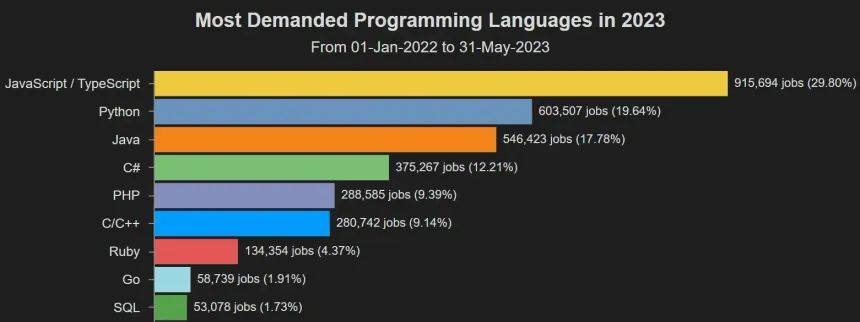
\includegraphics[width=\linewidth]{img/prog_languages_popularity.png}
    \caption{Lenguajes de programación más usados en 2023. Fuente: DevJobsScanner}
    \label{fig:prog-languages}
\end{figure}
En este proyecto, JavaScript se ha utilizado para diversos propósitos:

\begin{enumerate}
    \item \textbf{En el servidor:}
    \begin{itemize}
        \item \textbf{Manejo de rutas y archivos:} Se ha utilizado el framework Express.js para controlar el manejo de rutas y la creación de un servidor web. Express facilita la configuración del middleware para procesar solicitudes HTTP y servir archivos estáticos. En el código proporcionado Express se usa para definir rutas que manejan solicitudes tanto para la API como para la entrega de archivos HTML y recursos estáticos, como imágenes, CSS y JavaScript.
        \item \textbf{Manejo de archivos:} Se utilizan módulos nativos de Node.js para leer y escribir archivos. En el código se leen archivos JSON y HTML y se ayuda a resolver rutas de archivos y directorios, asegurando la correcta ubicación de los archivos en el sistema.
        \item \textbf{API de resultados:} Se implementan rutas para servir resultados de análisis almacenados en archivos JSON. Esto incluye la lectura de directorios y el envío de datos JSON a través de una API RESTful, que permite que el cliente recupere información sobre los resultados de forma dinámica.
    \end{itemize}
    
    \item \textbf{En el cliente:}
    \begin{itemize}
        \item \textbf{Manipulación del DOM:} JavaScript se usa para modificar dinámicamente el contenido y estilo de la página web según los datos recibidos del servidor. Por ejemplo, se crean y actualizan elementos HTML, se gestionan tablas y se aplican estilos en función de las propiedades de los datos.
        \item \textbf{Interactividad:} Se implementan funcionalidades interactivas como la ordenación de tablas y la actualización dinámica de contenido. Estas tablas se pueden ordenar basándose en las interacciones del usuario y se ocultan o muestran elementos de la interfaz según los datos recibidos.
        \item \textbf{Llamadas a la API:} El código del cliente realiza solicitudes HTTP a la API del servidor. Los datos devueltos se utilizan para iniciar o actualizar la interfaz de usuario, mostrando información relevante sobre los repositorios y sus resultados de análisis.
    \end{itemize}
\end{enumerate}

En resumen, el papel de JavaScript en este proyecto es crucial tanto en el lado del servidor como en el del cliente. La integración con Express y la manipulación dinámica del DOM (Document Object Model) permiten una experiencia de usuario fluida, cómoda y eficiente con los datos almacenados. Esta combinación de tecnologías ayuda a que la aplicación web sea interactiva, receptiva y funcional, cumpliendo con los estándares modernos de desarrollo web.

\section{Node.js}
Node.js es un entorno de ejecución diseñado para ejecutar código JavaScript en el lado del servidor. Node.js ha ganado popularidad debido a su capacidad para crear aplicaciones escalables y su extenso ecosistema de paquetes, accesible a través de npm (Node Package Manager).

En este proyecto Node.js ha sido empleado como el entorno principal para el servidor frontend, permitiendo ejecutar el código de visualización de resultados y gestionar las interacciones con la interfaz web. Se utilizó para:

\begin{enumerate}
    \item \textbf{Ejecución de código de frontend:} Node.js ejecuta el código que gestiona la lógica del servidor, incluyendo la carga de archivos y la configuración de la API.
    \item \textbf{Interacción con Express.js:} Node.js permite la integración con Express.js para manejar las rutas y las solicitudes HTTP, ofreciente una plataforma robusta para el desarrollo del servidor.
    \item \textbf{Manejo de datos:} La arquitectura no bloqueante de Node.js es clave para manejar eficientemente grandes volúmenes de datos, optimizando el rendimiento del servidor.
\end{enumerate}

\section{Express}
Express es un framework web minimalista para Node.js, diseñado para crear aplicaciones web y APIs de manera sencilla y eficiente. Nos ofrece una estructura flexible y una serie de herramientas que nos permiten gestionar rutas, peticiones HTTP y el middleware necesario para agregar funcionalidades adicionales a una aplicación. Al ser ligero y altamente configurable Express resulta ideal para construir aplicaciones escalables y robustas en entornos de desarrollo modernos.

En el contexto de este proyecto Express ha sido fundamental para:

\begin{enumerate}
    \item \textbf{Definir rutas y middleware:} Express.js ha facilitado la configuración de rutas para manejar tanto la API como la entrega de recursos estáticos y dinámicos, permitiendo una correcta visualización de los resultados analizados.
    \item \textbf{Facilitar la comunicación cliente-servidor:} La integración de Express ha simplificado la gestión de las comunicaciones entre el cliente y el servidor, optimizando la entrega de datos y la actualización de la interfaz de usuario.
\end{enumerate}

\section{JSON}
JSON (JavaScript Object Notation) es un formato ligero de intercambio de datos cuya fortaleza radica en que es fácil de leer y escribir para los humanos, así como sencillo de interpretar y generar por las máquinas. Su estructura basada en pares clave-valor lo hace ideal para transportar datos entre un servidor y una aplicación web, o incluso entre distintos componentes de un mismo sistema. JSON es ampliamente utilizado en APIs y servicios web debido a su simplicidad y compatibilidad con múltiples lenguajes de programación.

Por ejemplo, si quisiéramos almacenar la información de una persona podríamos utilizar una estructura similar a:

\begin{figure} [h]
    \centering
    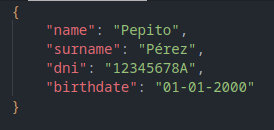
\includegraphics[height=4cm, keepaspectratio]{img/example_json.png}
    \caption{Ejemplo de objeto con formato JSON}
    \label{fig:enter-label}
\end{figure}

En este proyecto JSON ha sido crucial en dos aspectos:

\begin{enumerate}
    \item \textbf{Almacenamiento de los resultados:} Los resultados del análisis se almacenan en archivos JSON. Este formato ha permitido una organización clara y estructurada de los datos, facilitando su prosterior manipulación y visualización.
    \item \textbf{Intercambio de datos con la API de GitHub:} La información devuelta por las llamadas HTTP a la API de GitHub también está en formato JSON. Esto ha permitido integrar de manera eficiente los datos externos en el sistema, asegurando una comunicación fluida entre las distintas partes del proyecto.
\end{enumerate}

La capacidad ed JSON para representar objetos de manera sencilla ha sido esencial para la eficiencia y flexibilidad del proyecto.

\section{VSCode}
Visual Studio Code (VSCode) es un editor de código fuente desarrollado por Microsoft en abril de 2015. Desde entonces ha sido ampliamente adoptado por la comunidad de desarrolladores debido a su ligereza y versatilidad.

VSCode ofrece una experiencia de desarrollo robusta con características como resaltado de sintaxis, autocompletado inteligente, plena integración con Git y una muy amplia selección de extensiones para mejor la productividad y añadir funcionalidades.

En este proyecto VSCode ha sido empleado como el entorno principal de desarrollo debido a sus numerosas ventajas:

\begin{enumerate}
    \item \textbf{Soporte para múltiples lenguajes: } A diferencia de otras herramientas VSCode tiene la capacidad de manejar tanto JavaScript, como Python y otros lenguajes clave del proyecto. Esta flexibilidad ha sido de vital importancia para facilitar el trabajo con el backend, frontend y la manipulación de datos.
    \item \textbf{Extensiones y depuracicón: } Se han utilizado extensiones específicas para los lenguajes empleados, lo que ha facilitado y acomodado el proceso de desarrollo.
    \item \textbf{Integración con Git: } La integración nativa de Git en VSCode ha permitido gestionar fácilmente el control de versiones del proyecto, permitiendo recuperar de manera sencilla trozos de código que han sido editados.
\end{enumerate}

En definitiva, la flexibilidad y ligereza de VSCode lo convierte en una herramienta esencial para el desarrollo ágil y eficiente del proyecto, ayudando a mantener un flujo de trabajo organizado y estable.

\section{GitHub}

GitHub es una plataforma que facilita la gestión de proyectos utilizando Git, un sistema de versiones más extendido. Permite almacenar código en repositorios, donde varios desarrolladores pueden colaborar sin sobrescribir los cambios de otros mediante el uso de varias ramas, entre otras funcionalidades. 

En este proyecto se ha utilizado GitHub para gestionar las versiones de código, teniendo la capacidad de retroceder, ver y recuperar cambios realizados con anterioridad. Además, puesto que el programa desarrollado tiene como objetivo realizar análisis de repositorios alojados en GitHub, hemos utilizado también la API que proporciona para obtener información relevante de los mismos.

\section{Trello}
Trello es una herramienta de gestión de proyectos basada en el navegador que utiliza la metodología Kanban, la cual permite organizar tareas de forma visual e intuitiva mediante un sistema de tableros, listas y tarjetas. Los usuarios pueden mover tarjetas entre columnas para reflejar el estado de una tarea, facilitando la visualización del progreso de proyectos.

En este proyecto Trello ha sido utilizado para organizar las diferentes etapas de desarrollo, permitiendo mantener un registro de todas las tareas a realizar y el estado de las mismas. 

\begin{figure} [H]
    \centering
    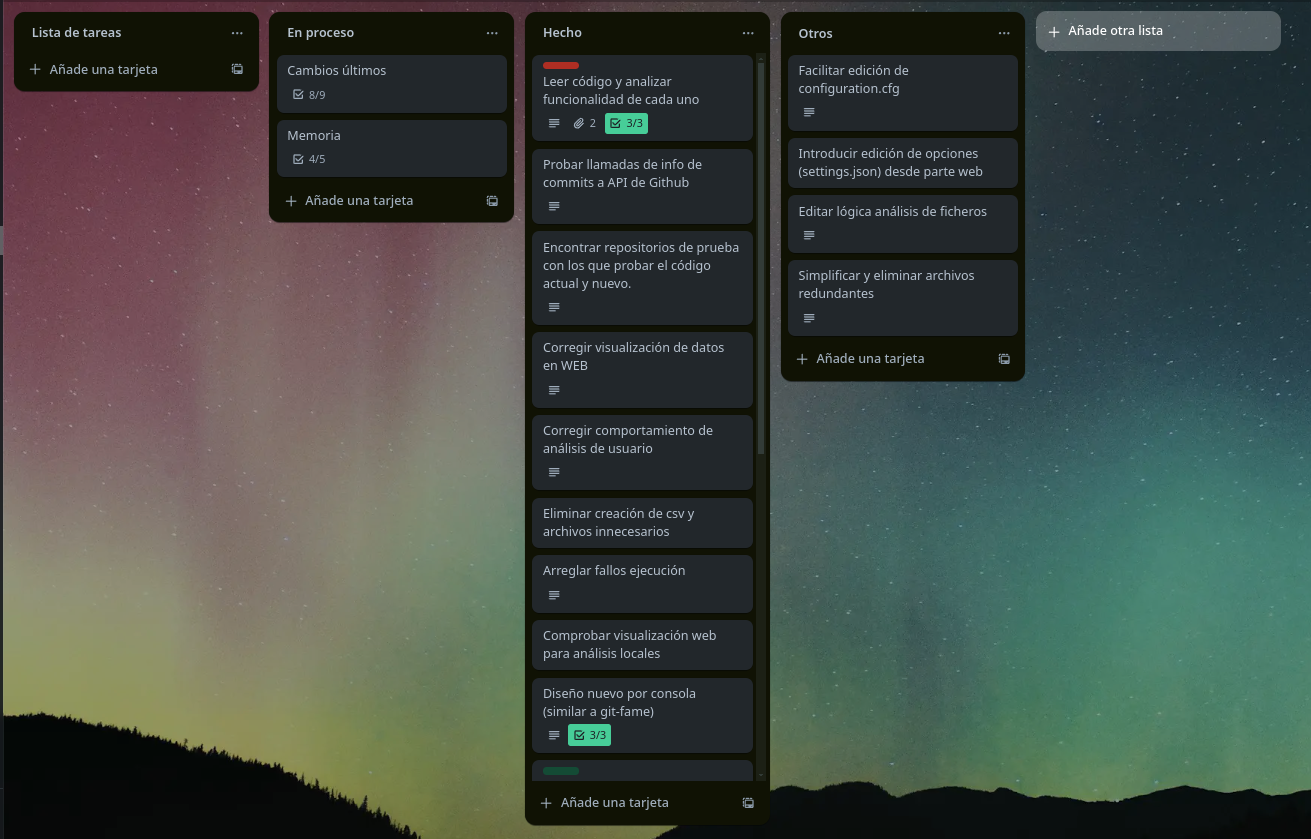
\includegraphics[width=\linewidth]{img/trello_example.png}
    \caption{Tablero de Trello utilizado}
    \label{fig:trello_example}
\end{figure}

En la figura 3.3 podemos ver el tablero de Trello empleado durante este proyecto, incluyendo muchas de las tarjetas empleadas distribuir las tareas a realizar.

\section{Postman} 
Postman es una herramienta utilizada para probar y desarrollar APIs, que permite a los desarrolladores enviar peticiones HTTP a un servidor y verificar las respuestas de manera intuitiva. Su interfaz gráfica facilita la creación de peticiones \texttt{GET}, \texttt{POST}, \texttt{PUT}, \texttt{DELETE}, entre otras, y ofrece funcionalidades avanzadas como la creación de colecciones, pruebas automáticas y la posibilidad de compartir entornos de trabajo.

En el contexto de este proyecto, Postman ha sido utilizado para:

\begin{enumerate}
    \item \textbf{Pruebas de APIs:} Se realizaron pruebas exhaustivas de las APIs desarrollados con Express y Node.js. Postman permitió verificar que las respuestas fueran correctas y que los datos se gestionaran adecuadamente en cada punto de la comunicación entre el cliente y el servidor.
    \item \textbf{Depuración y optimización:} La herramienta facilitó la identificación de errores y la optimización del rendimiento de las APIs. Su uso fue fundamental para asegurar la robustez y la funcionalidad de los endpoints antes de su implementación final.
\end{enumerate}

Postman ha sido de especial importancia para garantizar la calidad y fiabilidad del sistema al permitir una evaluación detallada de cada llamada HTTP realizada.

\section{Pycefr}

Pycefr es una herramienta de análisis de código Python, que permite realizar análisis de repositorios de código alojados en GitHub. Para ello descarga el código y recaba los elementos de Python existentes, otorgándoles una puntuación siguiendo el estándar CEFRL (Common European Framework of Reference for Languages).

Realizado el análisis, obtenemos varios archivos de resultados. Pycefr otorga también la posibilidad de crear archivos HTML con el objetivo de facilitar la visualización de estos resultados, listándonos todos los elementos encontrados junto con su respectiva puntuación.

Pycefr sido de especial relevancia en este proyecto, pues el propósito de éste ha sido su rediseño y extensión.


\label{sec:seccion1}

% Hemos hablado de cómo incluir figuras.
% Pero no hemos dicho nada de tablas.
% A mí me gustan las tablas.
% Mucho.
% Aquí un ejemplo de tabla, la Tabla~\ref{tab:ejemplo} (siento ser pesado, pero nota cómo he puesto la referencia).

% \begin{table}
 % \begin{center}
  % \begin{tabular}{ | l | c | r |} % tenemos tres colummnas, la primera alineada a la izquierda (l), la segunda al centro (c) y la tercera a la derecha (r). El | indica que entre las columnas habrá una línea separadora.
    % \hline
    % Uno & 2 & 3 \\ \hline % el hline nos da una línea vertical
    % Cuatro & 5 & 6 \\ \hline
    % Siete & 8 & 9 \\
    % \hline
  % \end{tabular}
  % \caption{Ejemplo de tabla. Aquí viene una pequeña descripción (el \emph{caption}, el pie de tabla/figura) del contenido de la tabla. Si la tabla no es autoexplicativa, siempre viene bien aclararla aquí.}
  % \label{tab:ejemplo}
 % \end{center}
% \end{table}

% Hay un sitio en Internet donde puedes diseñar las tablas fácilmente y luego hacer un corta y pega del resultado en tu editor.
% Puedes probarlo en \url{https://www.tablesgenerator.com/}.



%%%%%%%%%%%%%%%%%%%%%%%%%%%%%%%%%%%%%%%%%%%%%%%%%%%%%%%%%%%%%%%%%%%%%%%%%%%%%%%%
%%%%%%%%%%%%%%%%%%%%%%%%%%%%%%%%%%%%%%%%%%%%%%%%%%%%%%%%%%%%%%%%%%%%%%%%%%%%%%%%
% DISEÑO E IMPLEMENTACIÓN %
%%%%%%%%%%%%%%%%%%%%%%%%%%%%%%%%%%%%%%%%%%%%%%%%%%%%%%%%%%%%%%%%%%%%%%%%%%%%%%%%

\cleardoublepage
\chapter{Diseño e implementación}
\label{sec:diseno}

\section{Arquitectura general} 
\label{sec:arquitectura}

El objetivo de este proyecto es corregir y extender la funcionalidad, así como añadir una visualización web cómoda e intuitiva de los resultados obtenidos. Para ello hemos seguido los siguientes pasos:

\section{Obtención y comprensión del código existente}

El primer paso es muy básico pero indispensable. Debemos realizar una copia del repositorio original para obtener así un código del que partir que podamos modificar sin alterar el original. Una tarea no complicada que quedó solventada rápidamente mediante el uso de Git y GitHub. Hecho esto, podemos ponernos manos a la obra y comenzar a trabajar en el que a partir de ahora será nuestro código.

La mejor manera de comprender rápidamente qué hace un programa es ejecutándolo e ir, mediante ingeniería inversa, extrayendo qué está ocurriendo a medida que avanza la ejecución. Sin embargo, al intentar esto nos encontramos con que el programa presentaba una gran cantidad de errores y ni siquiera realizaba la labor que supuestamente debía. 

De este modo, hubo que virar el enfoque hacia una tarea diferente, volviéndose primordial el conseguir que el programa funcionase. Esto supuso un reto, porque en este punto todavía no estaba familiarizado con el código y desconocía qué debía hacer suponiendo que hiciese lo que debía, lo cual no era el caso.

\section{Creación de un registro de tareas}

El siguiente paso fue crear un nuevo tablero de Trello, del cual ya hemos hablado, para comenzar a recoger las tareas que iban apareciendo. Al principio del desarrollo estas tareas eran tan básicas como ``Revisión y comprensión del código'' y se volverían más específicas a medida que aumentara nuestro conocimiento sobre el proyecto.

Se realizaron diagramas de flujo para representar los proceso, con el fin de intentar entender y dejar anotado qué se realiza, dónde y cuándo.

\section{Solución de problemas de ejecución}

Comencé a editar pequeños fragmentos de código, a fin de intentar solucionar lo que pensaba en ese momento que eran los errores que impedían la correcta ejecución, pero a medida que unos se resolvían otros aparecían. Finalmente opté por rehacer el grueso del proyecto, dejando intacto de momento únicamente el proceso de análisis, es decir, la parte del programa que, dado cierto texto con código, lee y clasifica los elementos relacionados con Python que encuentra en el mismo.

De la parte del proyecto encargada se tomar y analizar los archivos sólo parecía funcionar (no daba error al instante) una de las tres opciones, la de analizar un repositorio dado un enlace de GitHub. Las otras dos, analizar un usuario de GitHub y analizar un directorio local, las dejé temporalmente de lado para centrarme en la primera. Si lograba hacer funcionar una de ellas, las otras dos no debían ser muy diferentes.

Toda esta parte conforma lo que en el proyecto he denominado ``backend'', dando a entender que es el código encargado de hacer el procesamiento y cálculos necesarios para obtener los resultados. La otra gran parte del proyecto, el llamado ``frontend'', sufría el mismo problema y daba errores de ejecución. De nuevo opté por rehacer el archivo principal que manejaba esa parte, obteniendo así unas primeras versiones ejecutables del código.

\section{Reestructuración y mejoras preparativas}

Una vez establecida una base ejecutable realicé unas últimas revisiones al código para asegurar el entendimiento del mismo. Además, antes de comenzar a implementar las nuevas funcionalidades se realizaron múltiples mejoras para facilitar el trabajo futuro:

\begin{itemize}
    \item Renombramiento y reelaboración de funciones para adecuarse a los estándares y simplificar su edición a futuros usuarios, utilizando nombres más representativos que expliquen rápidamente su finalidad.
    \item Añadida documentación.
    \item Reestructuración general del proyecto, diferenciando el código de backend y frontend en sus respectivas carpetas.
    \item Añadidos archivos de requisitos que el usuario puede utilizar para instalar rápidamente todo lo necesario para ejecutar el proyecto.
    \item Añadidos logs para que el usuario sepa en todo momento qué está realizando el programa. La demora del análisis en proyectos de gran tamaño pueden dar a entender al usuario que se ha parado cuando no es así. Estos logs vienen acompañados de mensajes de error descriptivos que indican al usuario por qué ha fallado el programa en caso de hacerlo.
\end{itemize}

\section{Implementación de nuevas funcionalidades}

Establecidas estas mejoras podemos comenzar a implementar desarrollos que extiendan las funcionalidades del proyecto actual. Puesto que el proyecto consta de dos grandes ramas, las agruperos de acorde a cuál de éstas pertenecen:

\subsection{Backend}

En lo relativo al backend encontramos la parte del proyecto encargada de procesar el input del usuario con el fin de recabar los datos necesarios y realizar el análisis que convenga. Los cambios más relevantes en esta parte son los siguientes:

\begin{itemize}
    \item \textbf{Extensión del análisis del repositorio }, incluyendo información relevante sobre el historial del mismo y de los usuarios que han participado en él. En caso de analizar un directorio local el programa comprobará antes si forma parte de un repositorio en GitHub. En caso de ser así, preguntará al usuario si prefiere analizar directamente el repositorio en cuestión en lugar de los archivos locales. Las ventajas que tiene esto son (1) el directorio local puede no estar actualizado con los últimos cambios subidos al repositorio, de modo que al analizar directamente la versión de GitHub nos aseguramos de estar analizando la última versión compartida, y (2) nos añade a los resultados del análisis esa información referente a GitHub, en lugar de únicamente la del código.

    \item \textbf{Mejora del archivo resultante del análisis} para facilitar su posterior tratamiento. Originalmente se generaban dos archivos equivalentes en formatos JSON y CSV. Aunque ambos formatos son ampliamente utilizados para el análisis de datos, hemos optado por mantener únicamente el formato JSON debido a su mayor flexibilidad para estructurar y manipular información. A diferencia del CSV, que se ajusta mejor a datos tabulares con campos claramente definidos y fijos, el JSON permite cambios más dinámicos en la estructura de los datos sin la necesidad de realizar ajustes constantes para que los campos se adapten a un formato rígido. Esto hace que el JSON sea más adecuado para futuras reestructuraciones del archivo, evitando la complejidad asociada a modificar archivos CSV cuando la estructura de los datos cambia significativamente. Al prescindir del archivo CSV, simplificamos el proceso de manejo y actualización de los datos, permitiendo una mayor versatilidad en su tratamiento y reduciendo las dificultades asociadas al ajuste de formatos estáticos como el CSV.

    \item \textbf{Añadida visualización de resultados desde la terminal}, en caso de que el usuario prefiera una vista rápida de los resultados sin tener que depender de la parte web. 
\end{itemize}

\clearpage

\begin{figure}[H]
  \centering
  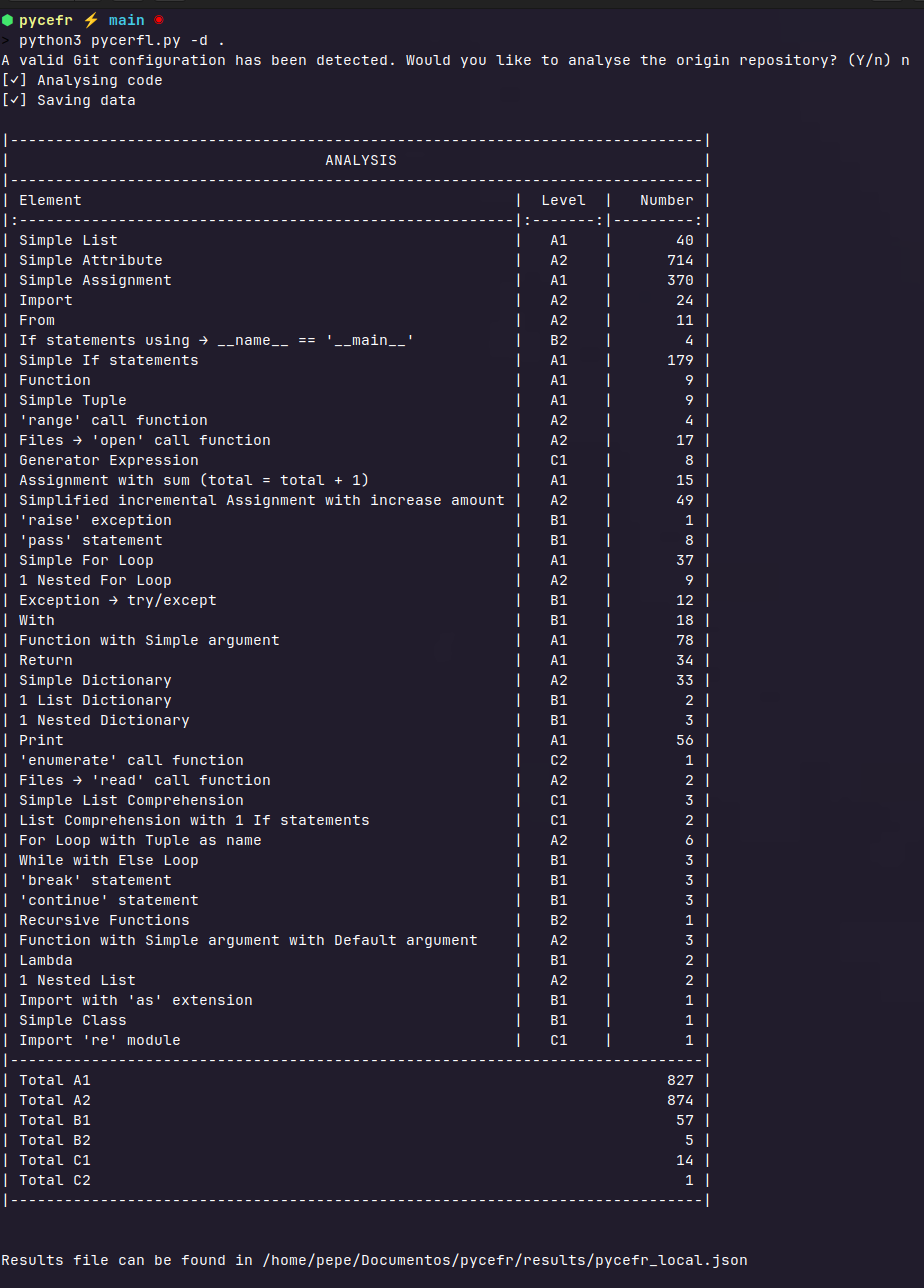
\includegraphics[width=\linewidth, keepaspectratio]{img/execution_local.png}
  \caption{Vista de resultados por consola tras análisis de directorio local}
  \label{fig:execution_local}
\end{figure}

\begin{figure}[H]
  \centering
  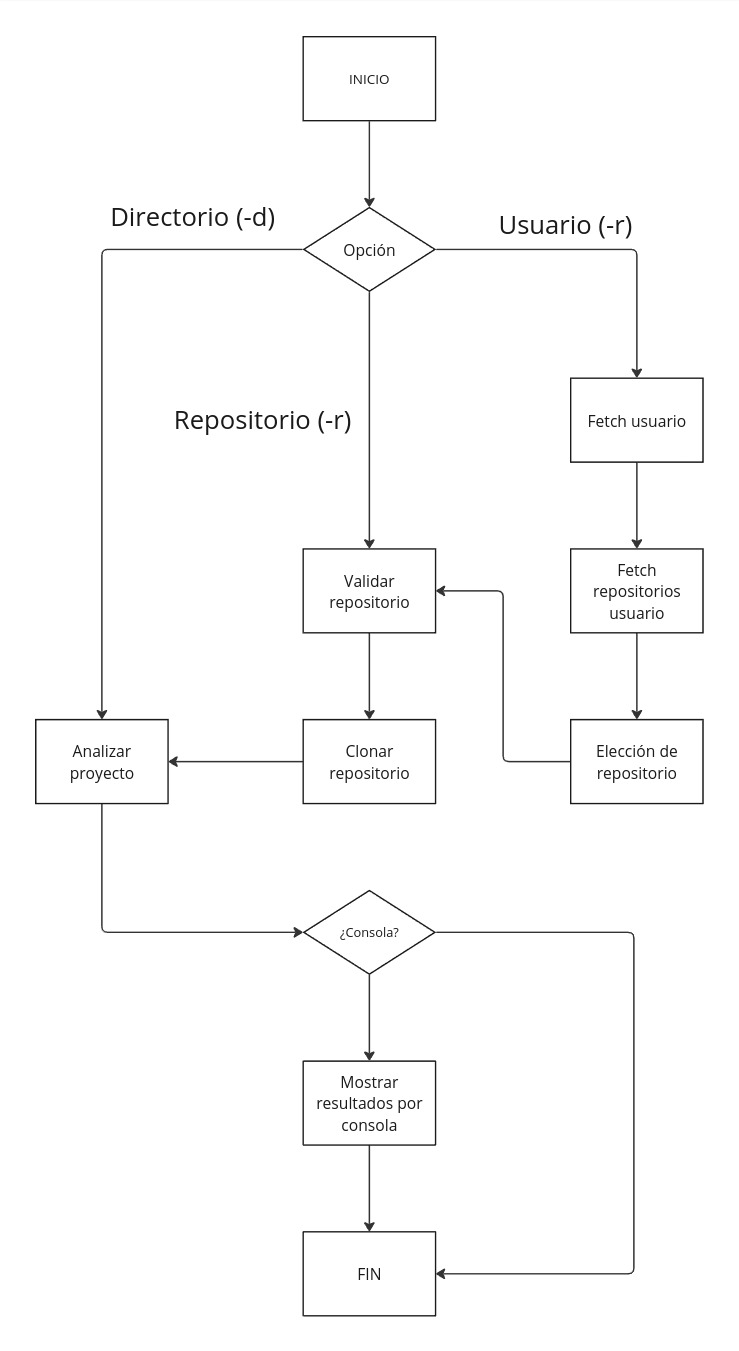
\includegraphics[height=\textheight, keepaspectratio]{img/esquema_backend_final.jpg}
  \caption{Flujo del backend (análisis)}
  \label{fig:execution_local}
\end{figure}

En la figura 4.1 podemos ver un ejemplo de ejecución del análisis de un directorio local. Introducimos la opción \textit{-d} para analizar un directorio local, y la dirección \textit{``,''} para referirnos al repositorio en que nos encontramos actualmente, esto es, el de la propia aplicación. 

Se nos muestra un primer mensaje indicando que se ha encontrado una configuración Git válida, preguntándonos si estamos interesados en analizar el repositorio original. Este mensaje se corresponde con el primer paso del flujo de ejecución mostrado en la figura 4.2. Se comprueba si el código contiene información relativa a Git, y en caso de ser así, da al usuario la opción de analizar el repositorio directamente de GitHub, en lugar de analizar el directorio local. En este ejemplo se ha indicado al programa que no, de modo que procede con el análisis del proyecto, mostrando los pasos realizados \textit{"Analysing code"} y \textit{"Saving data"}, y finalmente los resultados por consola.

Finalmente se añadieron también otras dos opciones de ejecución: La primera de éstas es 

\begin{itemize}
    \item \textbf{Consola (-c)} para imprimir por consola resultados ya existentes, sin necesidad de realizar de nuevo el proceso de análisis.
    \item \textbf{Lista (-l)} para listas los archivos de resultados ya existentes.
\end{itemize}

De este modo, en cualquier momento el usuario puede obtener un listado de los resultados ya existentes y visualizar por consola uno de ellos mediante la siguiente secuencia de comandos:

\begin{verbatim}
    python3 pycefrl.py -l
    python3 pycefrl.py -c <RESULTADOS>
\end{verbatim}

\subsection{Frontend}

Utilizamos el término ``frontend'' para la parte del proyecto encargada de la web. En nuestro caso usamos la web para la navegación y visualización de los archivos producidos como resultado de los análisis.

La versión original del frontend es funcional, en el sentido de que cumple su labor, pero presentaba una estructura muy básica y poco modular. Todo el código relevante estaba contenido en un único archivo `main.js`, que generaba dinámicamente un archivo HTML a partir de unas plantillas e insertaba directamente toda la información en la página. Esto no solo dificultaba la escalabilidad del proyecto, sino que también limitaba la separación de responsabilidades entre las diferentes partes del frontend y hacía más complicado el mantenimiento del código a largo plazo.

En este rediseño completo del frontend hemos implementado una estructura más profesional y escalable. Se han organizado los recursos del proyecto en carpetas separadas, como `public`, `assets`, `html`, `css` y `js`, siguiendo las buenas prácticas del desarrollo web moderno. Asimismo, se ha incluido un archivo `package.json`, fundamental para gestionar las dependencias del proyecto y definir los scripts necesarios para su ejecución. El uso de `npm` como gestor de dependencias permite que el proyecto sea fácilmente reproducible en cualquier entorno, garantizando que todas las bibliotecas y módulos requeridos puedan ser instalados de manera automática y coherente.

Para el servidor, hemos adoptado `Express.js` como framework, creando un archivo `server.js` dedicado a cargar y gestionar el servidor web, lo que no existía en la versión anterior. También se han implementado rutas específicas para la API (`apiRoutes.js`) y para servir las páginas HTML (`htmlRoutes.js`), lo que proporciona una clara separación entre la lógica de backend y la presentación de los datos. Esto mejora el manejo de peticiones y la organización del código, haciendo más eficiente la gestión del servidor y la comunicación entre las distintas capas de la aplicación.

Además, el uso del `package.json` facilita la futura definición de scripts para tareas comunes como la ejecución del servidor en modo desarrollo, la instalación de dependencias y el despliegue. Esto asegura que todos los colaboradores del proyecto puedan utilizar los mismos comandos y configuraciones, evitando problemas derivados de configuraciones locales.

En resumen, este rediseño transforma el frontend en un proyecto más modular, mantenible y alineado con estándares profesionales, lo que facilita tanto su evolución futura como la colaboración en equipo. La inclusión de `Express.js`, junto con el uso de `npm` y un `package.json` bien definido, asegura que la gestión de dependencias y la ejecución del proyecto sean eficientes y consistentes.

A continuación podemos observar el cambio significativo en la estructura del frontend tras el rediseño. La figura 4.3 muestra el árbol de archivos original, donde todo el código estaba contenido en un único archivo `main.js`. Por el contrario, la figura 4.4 ilustra el nuevo diseño, que adopta una estructura modular y organizada en carpetas, incluyendo archivos específicos para las rutas de la API, los estilos, los scripts, y el uso de `Express.js` para la gestión del servidor.


\vspace{2em}
\begin{figure}[htbp]
  \centering
  \begin{minipage}[t]{0.35\textwidth}
    \centering
    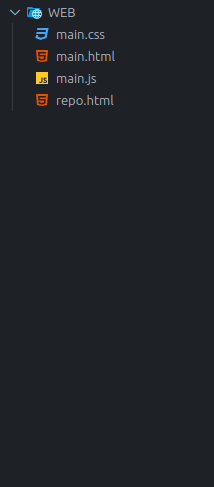
\includegraphics[width=\textwidth, keepaspectratio]{img/tree_frontend_original.png}
    \caption{Estructura original del frontend}
    \label{fig:original_structure}
  \end{minipage}
  \hspace{0.1\textwidth}
  \begin{minipage}[t]{0.35\textwidth}
    \centering
    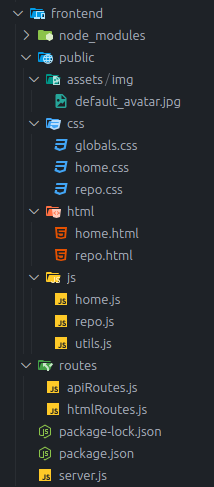
\includegraphics[width=\textwidth, keepaspectratio]{img/tree_frontend_final.png}
    \caption{Nueva estructura del frontend tras el rediseño}
    \label{fig:new_structure}
  \end{minipage}
\end{figure}

Toda esta reestructuración implica naturalmente un cambio absoluto en el funcionamiento de esta sección. En las siguientes imágenes podemos ver una comparativa de ambos flujos de trabajo:

\begin{figure}[H]
    \centering
    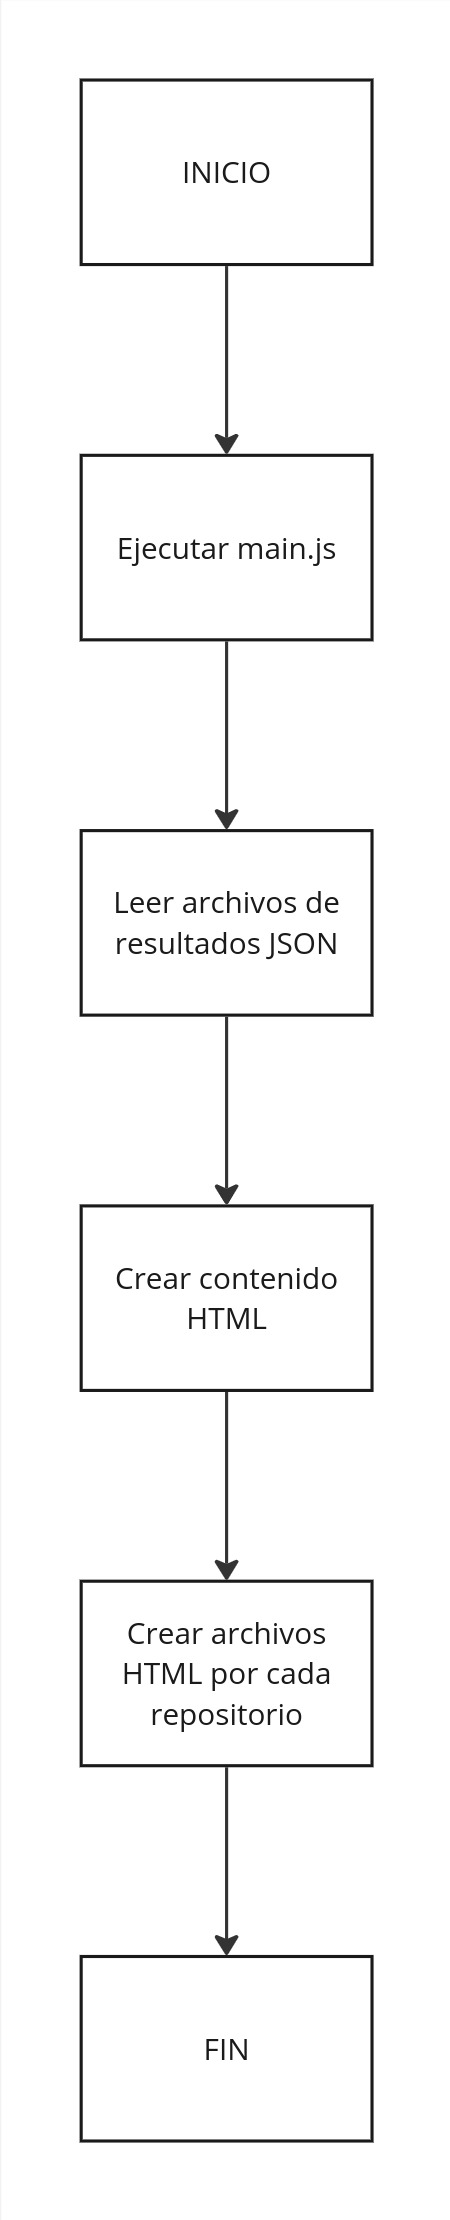
\includegraphics[height=19cm, keepaspectratio]{img/esquema_frontend_original.jpg}
    \caption{Flujo del frontend original}
    \label{fig:original_frontend}
\end{figure}
\begin{figure} [H]
    \centering
    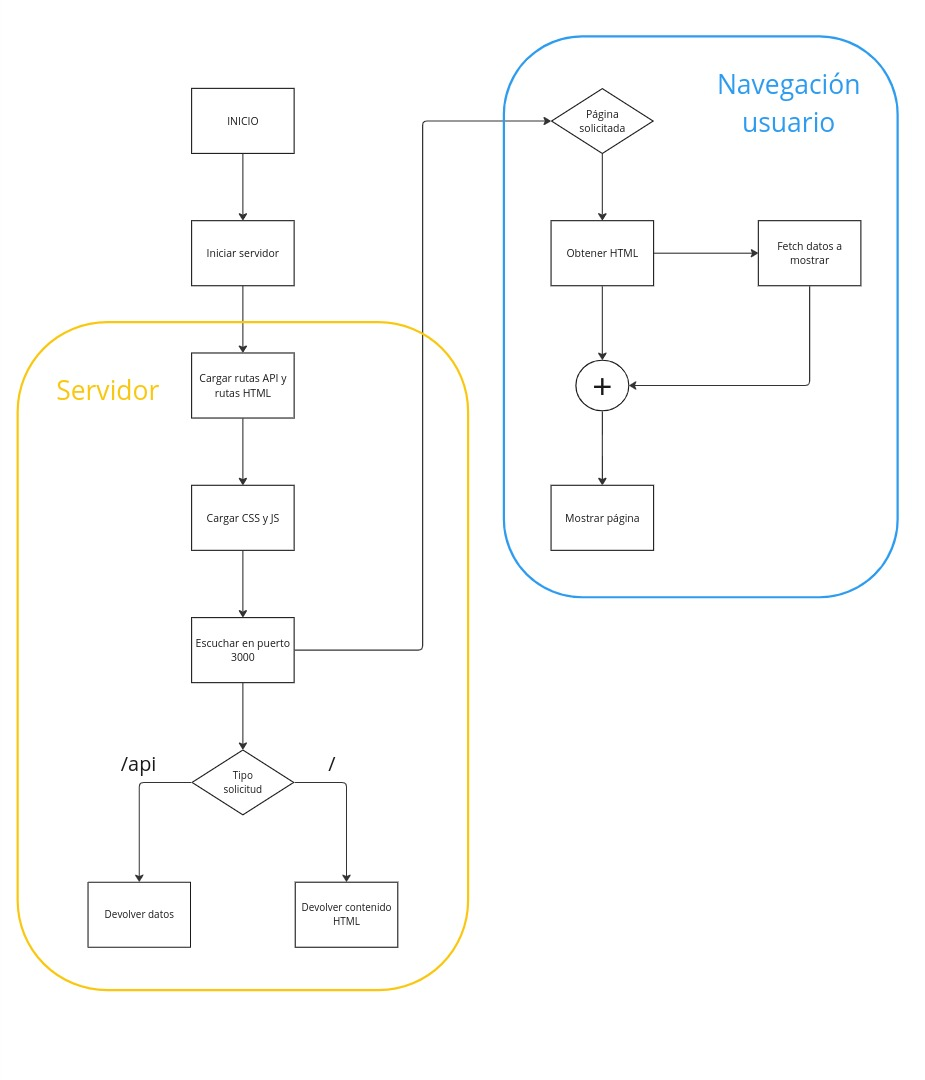
\includegraphics[width=\textwidth, height=\textheight, keepaspectratio]{img/esquema_frontend_final.jpg}
    \caption{Flujo del frontend rediseñado}
    \label{fig:final_frontend}
\end{figure}

En el \textbf{flujo original}, que podemos ver en la figura 4.5, ejecutamos casi exclusivamente el archivo 'main.js', el cual realiza todo el trabajo. Éste busca en el sistema archivos de resultados JSON y extrae de ellos la información relevante a mostrar. Tras esto carga unas plantillas para crear dos archivos HTML:

\begin{itemize}
    \item Un archivo 'index.html' que consta de un breve resumen de la información los análisis realizados. Desde aquí se puede acceder a cada análisis individual.
    \item Un archivo '\textit{nombreDelRepositorioAnalizado}.html' que incluye todo el análisis realizado en el repositorio correspondiente.
\end{itemize}

Una vez creados podemos visualizarlos levantando un servidor local, aunque esto no es algo incluido en el proceso original, sino que hacerlo por nosotros mismos.

En \textbf{flujo actualizado} (ver figura 4.6) ha sido diseñado pensando en la flexibilidad y facilidad para una futura ampliación, añadiendo nuevos procesos y agrupando los ya existentes en archivos encargados de tareas comunes. Así, podemos definir los siguientes pasos en el proceso de ejecución:

\begin{enumerate}
    \item  Comenzamos ejecutando el archivo 'server.js', el cual crea y levanta un servidor que proporcionará todo el contenido necesario, tanto las páginas web como los resultados de los análisis. 
    
    \item El servidor se encarga de cargar la lógica de enrutamiento y la api, las cuales se encuentran cada una en sus respectivos archivos (htmlRoutes.js y apiRoutes.js), además de archivos encargados de los estilos y lógica de cada página web.

    \item El servidor comienza a escuchar, esto es, esperar a recibir solicitudes. En nuestro caso encontramos dos tipos de solicitudes: \textbf{solicitudes de datos} (se piden los resultados de uno o más análisis) y \textbf {solicitudes de páginas} (se pide al servidor el contenido HTML a mostrar en un momento determinado).

    \item El usuario puede ya comenzar a navegar. Al entrar en la dirección proporcionada por el servidor se dirigirá por defecto a la página principal, la cual incluye el resumen de los análisis existentes, incluyendo la información del repositorio GitHub en caso de incluirla.

    \item Al seleccionar uno de los resultados podrá ver toda la información del análisis seleccionado, además de información relevante del repositorio.
    
\end{enumerate}

En definitiva, uniendo ambas secciones, \textit{backend} y \textit{frontend}, obtenemos la siguiente arquitectura:

\begin{figure}
    \centering
    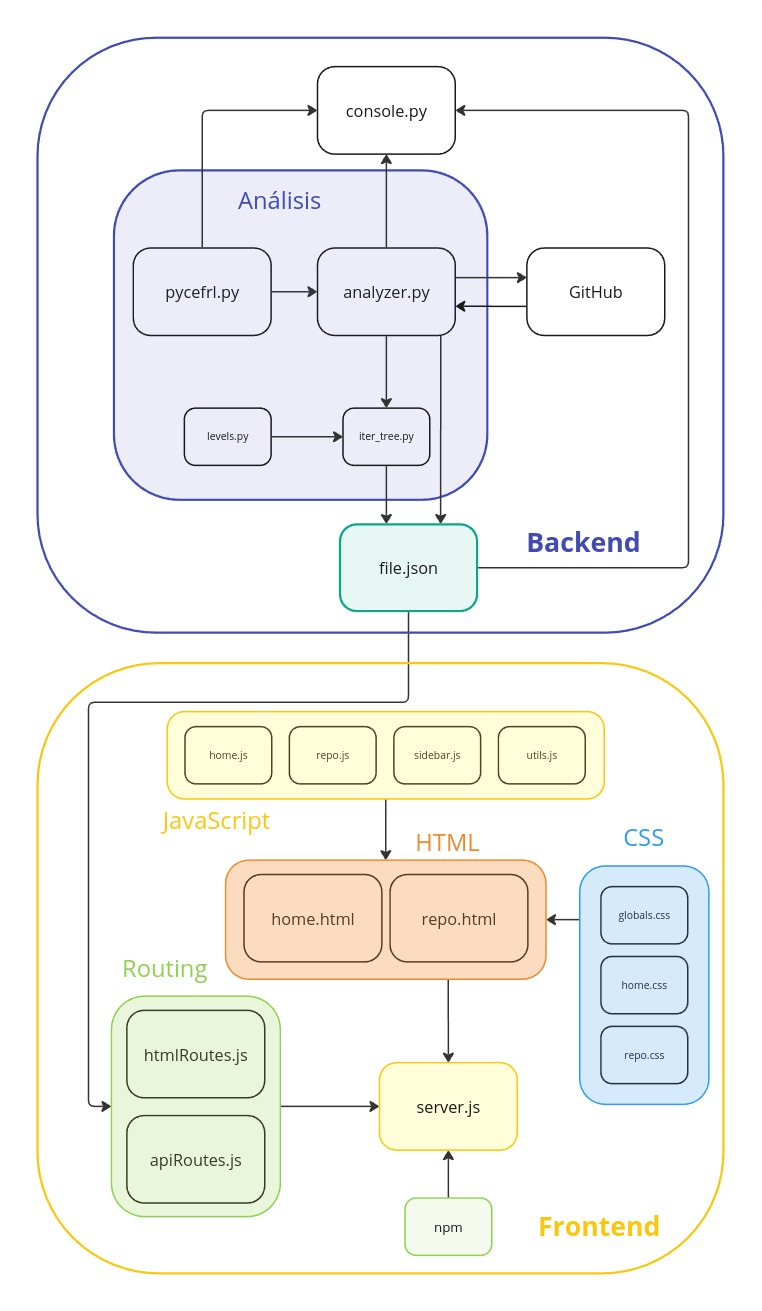
\includegraphics[height=\textheight]{img/arquitectura_total_final.jpg}
    \caption{Arquitectura del proyecto}
    \label{fig:enter-label}
\end{figure}

En la figura 4.7 podemos visualizar de manera esquemática la arquitectura del proyecto completo, agrupando los archivos involucrado no sólo por la sección a la que pertenecen sino por la tarea que cumplen.

El \textbf{backend} contiene los archivos utilizados para realizar el análisis del código. El archivo \textit{pycefrl.py} procesa la entrada del usuario. Interacciona directamente con el archivo \textit{console.py} en caso de que el usuario use el programa para visualizar datos ya existentes, puesto que éste es el archivo que procesa el mostrado de los resultados por consola. Sin embargo, durante su actividad más habitual, la del análisis de archivos, interactúa con \textit{analyzer.py}, quien realiza la gestión principal de este proceso de análisis, sirviéndose primero de la API de GitHub para obtener información en caso de necesitar, y segundo del archivo \textit{iter\_tree.py}, para navegar por el código Python a analizar. Éste a su vez se sirve de \textit{levels.py} para asignar los niveles correspondientes a los elementos Python encontrados, produciendo un archivo JSON con los resultados, cuyo nombre se corresponderá con el del proyecto analizado. Finalmente el \textit{analyzer.py} añade al JSON la información relativa a GitHub. 

En el \textbf{frontend} se incluyen todos los archivos involucrados en el funcionamiento del servidor web. El usuario debe simplemente ejecutar el archivo \textit{server.js}, y éste se encarga de manera automática de utilizar los archivos necesarios para cada tarea. En esta parte podemos diferencer varios grupos de archivos:

\begin{itemize}
    \item \textbf{Routing:} Archivos encargados de procesar las solicitudes HTTP. \textit{apiRoutes.js} permite al servidor procesar las solicitudes a API, normalmente devolviendo datos en la respuesta. El archivo \textit{htmlRoutes.js} permite al servidor devolver el contenido HTML que mostrar en cada situación. Toda la información de este grupo de archivos depende de los archivos de resultados, los cuales son leídos para devolver la información pertinente.

    \item \textbf{JavaScript:} Archivos JavaScript que contienen la lógica utilizada por los archivos HTML.

    \item \textbf{CSS:} Archivos CSS que definen los estilos de las páginas. Son empleados también por los archivos HTML.
    
    \item \textbf{HTML:} Archivos HTML que conforman las plantillas de las páginas mostradas. Utilizan la lógica de los archivos JavaScript para obtener los datos y mostrarlos en la página, y aplican los estilos espeficiados en los archivos CSS indicados.

    \item \textbf{npm:} Incluye los módulos de Node.js utilizados en el proyecto.
\end{itemize}

 
%Recuerda que toda figura que añadas a tu memoria debe ser explicada.
%Sí, aunque te parezca evidente lo que se ve en la figura~\ref{fig:arquitectura}, la figura en sí solamente es un apoyo a tu texto.
%Así que explica lo que se ve en la figura, haciendo referencia a la misma tal y como ves aquí.
%Por ejemplo: En la figura~\ref{fig:arquitectura} se puede ver que la estructura del \emph{parser} básico, que consta de seis componentes diferentes: los datos se obtienen de la red, y según el tipo de dato, se pasará a un \emph{parser} específico y bla, bla, bla\ldots

% Si utilizas una base de datos, no te olvides de incluir también un diagrama de entidad-relación.


%%%%%%%%%%%%%%%%%%%%%%%%%%%%%%%%%%%%%%%%%%%%%%%%%%%%%%%%%%%%%%%%%%%%%%%%%%%%%%%%
%%%%%%%%%%%%%%%%%%%%%%%%%%%%%%%%%%%%%%%%%%%%%%%%%%%%%%%%%%%%%%%%%%%%%%%%%%%%%%%%
% EXPERIMENTOS Y VALIDACIÓN %
%%%%%%%%%%%%%%%%%%%%%%%%%%%%%%%%%%%%%%%%%%%%%%%%%%%%%%%%%%%%%%%%%%%%%%%%%%%%%%%%

\cleardoublepage
\chapter{Validación y pruebas}
\label{chap:experimentos}

% Este capítulo se introdujo como requisito en 2019. 
% Describe los experimentos y casos de test que tuviste que implementar para validar tus resultados. 
% Incluye también los resultados de validación que permiten afirmar que tus resultados son correctos. 

La validación del código añadido o editado se ha ido realizando en la mayor parte de los casos durante la propia codificación. A menudo se han ido probando los cambios a medida que se implementaban en la medida de lo posible. Naturalmente, en la mayoría de ocasiones estas pruebas se hacían por bloques, y no ha sido hasta la fase final del desarrollo (último mes, mes y medio) que se comenzaron a hacer pruebas del proceso completo. Esto se debe a que desde el principio se ha tenido una idea de producto final que presentaba muchas incompatibilidades (en cuanto a código se refiere) con el producto original, y resulta inconveniente, además de una más que ineficiente inversión del tiempo de desarrollo, asegurar la compatibilidad completa de las partes en todo momento.

Como ya ha sido mencionado el comienzo del desarrollo consistió en la creación de una versión estable, puesto que en un principio nos encontramos con múltiples errores de ejecución. Se decidió también, de cara a facilitar la compresión del código, refractorizar gran parte de éste. Esta versión estable se tomó tras realizar los cambios justos y necesarios para solucionar aquellos procesos que producían los errores, y para poder acceder en el futuro rápidamente a ella (para poder comprobar en todo momento el funcionamiento original) se añadió con Git una rama local bajo del nombre ``original-fixed'' a partir del commit en que se subieron esos últimos cambios. Esto estableció el primer 'ancla' en el proyecto, proporcionándome un punto de referencia al que poder regresar si más adelante me encontrara con errores críticos difíciles de rastrear, además de permitirme realizar las primeras pruebas, aunque fuera del código original.

Tras esto los cambios se fueron probando poco a poco, a medida que se desarrollaban. Sin embargo, al introducir los cambios que incorporaban llamadas a la API de GitHub se me presentó la necesidad de probar dichas llamadas de algún modo. Ejecutar el análisis era una opción poco eficiente, dado que se perdería mucho tiempo ejecutando código cuando sólo estamos interesados en la llamada. En ocasiones muy concretas utilicé la herramienta \texttt{curl} desde la terminal, que me permite realizar solicitudes HTTP, pero resultaba incómoda cuando se trataba se llamadas complejas.

\vspace{1em}
\begin{figure}[H]
    \centering
    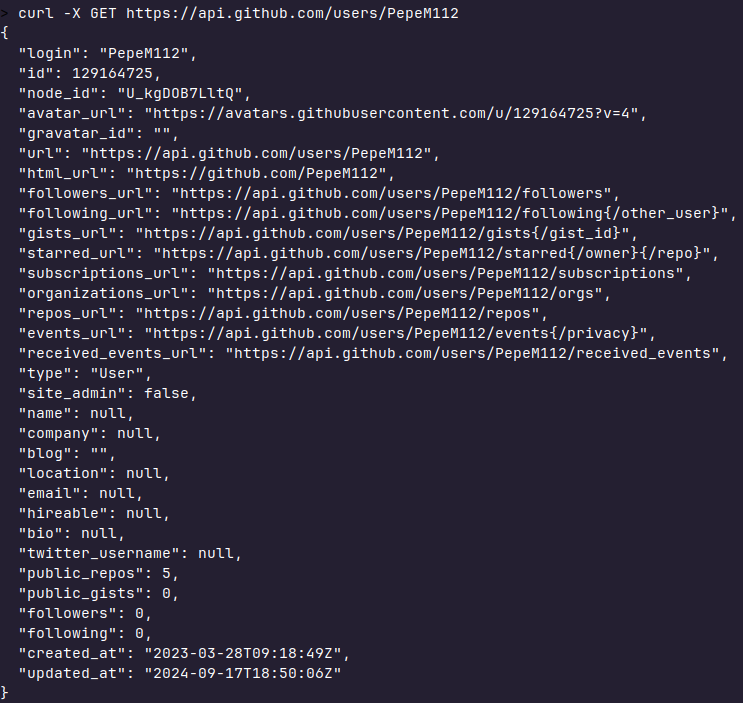
\includegraphics[width=15cm]{img/curl_example.png}
    \caption{Ejemplo de llamada con \textit{curl}}
    \label{fig:postman}
\end{figure}

Como podemos ver en la figura 5.1 la herramienta \texttt{curl} tiene como gran ventaja la agilidad que proporciona al poder ser utilizada desde la terminal, de modo que puede resultar de gran ayuda para consultas rápidas. Sin embargo, dado el número de llamadas que debía realizar a lo largo del proyecto realizar las pruebas de esta manera se volvía un proceso tedioso, sobre todo para llamadas más complejas. Además, una necesidad común durante el desarrollo fue querer acceder de nuevo a las respuestas de llamadas ya probadas anteriormente, obligando a tener que repetir la llamada de nuevo. Es por ello que opté por usar \textbf{Postman}.

Postman me proporcionó una interfaz para desarrollar y probar tanto la API de GitHub como la desarrollada por mí para el frontend. Creé una nueva colección que contendría todas las llamadas que se realizan en el proyecto. Esta herramienta me permite añadir y editar fácilmente solitudes que quiera realizar,con todo tipo de información. Además, permite guardar como ejemplos de ejecución de dichas llamadas, lo cual resolvió el problema de querer acceder de nuevo a los resultados de una llamada. Por ejemplo, a menudo necesitaba comprobar la estructura de la respuesta o el nombre del valor que quería extraer de ésta, y guardar de manera permanente estas respuestas me permitió satisfacer esta necesidad.

\vspace{2em}

\begin{figure}[H]
    \centering
    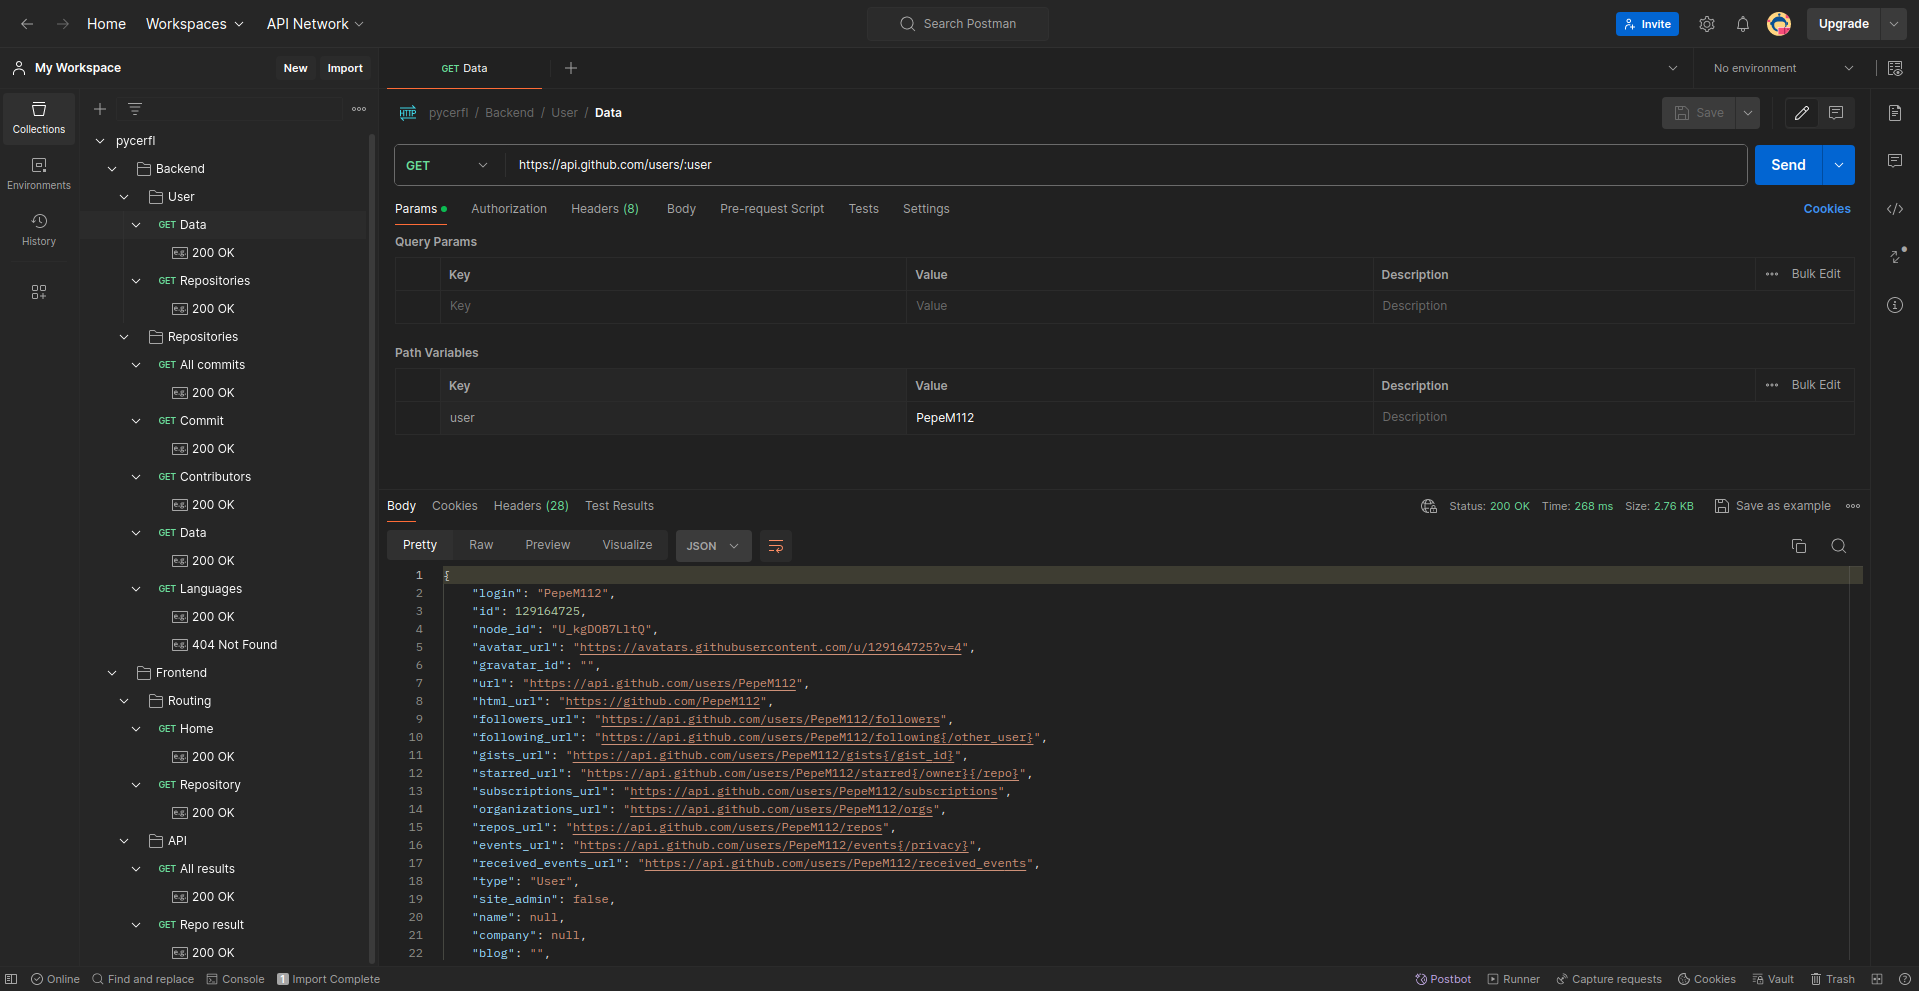
\includegraphics[width=\textwidth]{img/postman.png}
    \caption{Ejemplo de llamada con Postman}
    \label{fig:postman}
\end{figure}
\clearpage

En la figura 5.2 podemos ver la interfaz de Postman. En el lado izquierdo encontramos un árbol de la colección de llamadas utilizadas en el proyecto. Con esto podemos simplemente seleccionar la llamada que necesitamos, editarla con la información necesaria (bloque superior), hacerla y visualizar la respuesta (bloque inferior). Esto permitió obtener las respuestas a cualquier llamada de manera rápida y clara. Además, el formato empleado para las respuestas a las solicitudes es JSON, el cual, como ya hemos visto, permite una fácil manipulación de los datos.

En nuestro caso gran parte de las llamadas son a la API de GitHub, quien implementa medidas de seguridad que limitan las solicitudes desde una misma dirección IP si se detecta un número excesivo en un corto período de tiempo. Esto lo hace con el fin para prevenir abusos y proteger la plataforma de posibles ataques automatizados. Es por ello que se incluyó la opcion de incluir un token en el archivo de ajustes. En caso de que el usuario exceda el límite de solicitudes se le presentará un mensaje de error indicando qué debe hacer para solventar este problema, como se muestra en la figura 5.3: 

\vspace{1em}
\begin{figure}[H]
    \centering
    
\includegraphics[width=\textwidth]{img/results/backend_exe_r_api_error.png}
    \caption{Ejemplo de error por exceso de llamadas a la API}
    \label{fig:api_limit}
\end{figure}
\vspace{1em}

En un principio se incluyeron únicamente las llamadas que ahora se encuentran bajo la carpeta \textit{Backend}, pero en al retomar el desarrollo de la parte web surgió la necesidad de añadir las solicitudes realizadas aquí también. En este caso las llamadas son a nuestro propio servidor local que levantamos para mantener la página web, el cual funciona como una API REST y devuelve tanto los datos de los análisis en formato JSON como el HTML necesario para el renderizado de cada página.

Las pruebas finales consistieron en comprobar la correcta visualización de la parte web, lo cual consiste principalmente en levantar el servidor y navegar por las páginas, y finalmente comprobar el proceso completo, realizando primero un análisis y arrancando luego el servidor para comprobar que los datos se muestran en la web.

%%%%%%%%%%%%%%%%%%%%%%%%%%%%%%%%%%%%%%%%%%%%%%%%%%%%%%%%%%%%%%%%%%%%%%%%%%%%%%%%
%%%%%%%%%%%%%%%%%%%%%%%%%%%%%%%%%%%%%%%%%%%%%%%%%%%%%%%%%%%%%%%%%%%%%%%%%%%%%%%%
% RESULTADOS %
%%%%%%%%%%%%%%%%%%%%%%%%%%%%%%%%%%%%%%%%%%%%%%%%%%%%%%%%%%%%%%%%%%%%%%%%%%%%%%%%

\cleardoublepage
\chapter{Resultados}
\label{chap:resultados}

En este capítulo procederemos a ver ejemplos de uso de la aplicación. Para ello hemos tomado el repositorio https://github.com/wohlert/semi-supervised-pytorch. Se trata de un repositorio público de GitHub de un tamaño entre pequeño y moderado con el que se han ido realizando numerosas pruebas a lo largo del desarrollo del proyecto.

\section{Backend}

El backend consiste esencialmente en la ejecución del archivo \texttt{pycefr.py}. Éste consta de 5 posibles métodos de ejecución, los cuales podemos obtener rápidamente añadiendo el argumento -h o --help:

\vspace{2em}
\begin{figure}[htbp]
    \centering
    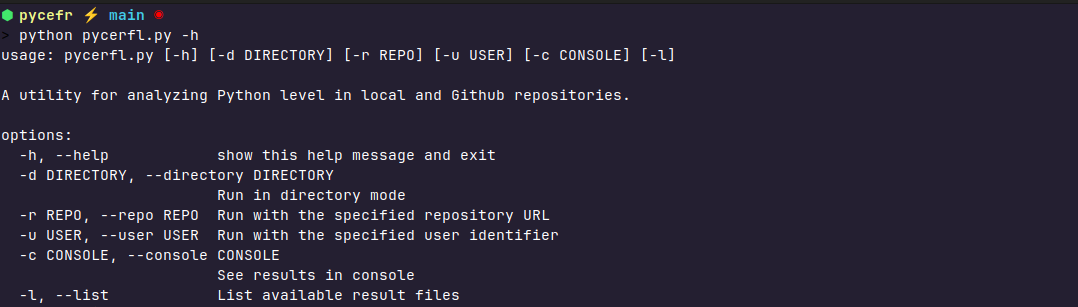
\includegraphics[width=\textwidth, keepaspectratio]{img/results/backend_exe_h.png}
    \caption{Ejemplo de uso de argumento help}
    \label{fig:analysis_help}
\end{figure}

En la figura 6.1 se nos muestra el resultado de ejecutar el programa utilizando este argumento -h para obtener ayuda sobre el uso de la aplicación. Comienza indicándonos el formato con que debemos ejecutarlo (usage). pycefrl.py es el archivo que queremos ejecutar, y cada uno de los corchetes siguientes indica un posible argumento a introducir, incluyendo en ocasiones segundos argumentos posibles, como es el caso de -d (DIRECTORY), -r (REPO), -u (USER) y -c (CONSOLE). Esto da a entender al usuario que en estos casos el programa espera un segundo argumento, el cual se corresponde en estos casos con el directorio (-d), repositorio (-r), usuario (-u) a analizar o el archivo de resultados a visualizar (-c).

Entendido esto, procederemos a explicar cada una de las opciones:

\subsection{Repositorio (-r)}

Utilizamos las opciones \texttt{-r <REPO\_URL>} para realizar un análisis de un repositorio remoto alojado en GitHub. 

Podemos ver el resultado de este análisis en la figura 6.2. Hemos introducido como segundo argumento el repositorio sobre el que vamos a realizar el análisis. Como en otros ejemplos hemos utilizado el proyecto \textit{semi-supervised-pytorch} del usuario ``wohlert''.

La consola nos muestra primero los mensajes de estado de cada proceso que realiza. Una vez terminado el proceso muestra por pantalla el resultado del análisis, lo cual se puede activar o desactivar editando el archivo de configuración \textit{settings.json}.
\newpage
\vspace{1em}

\begin{figure} [H]
    \centering
    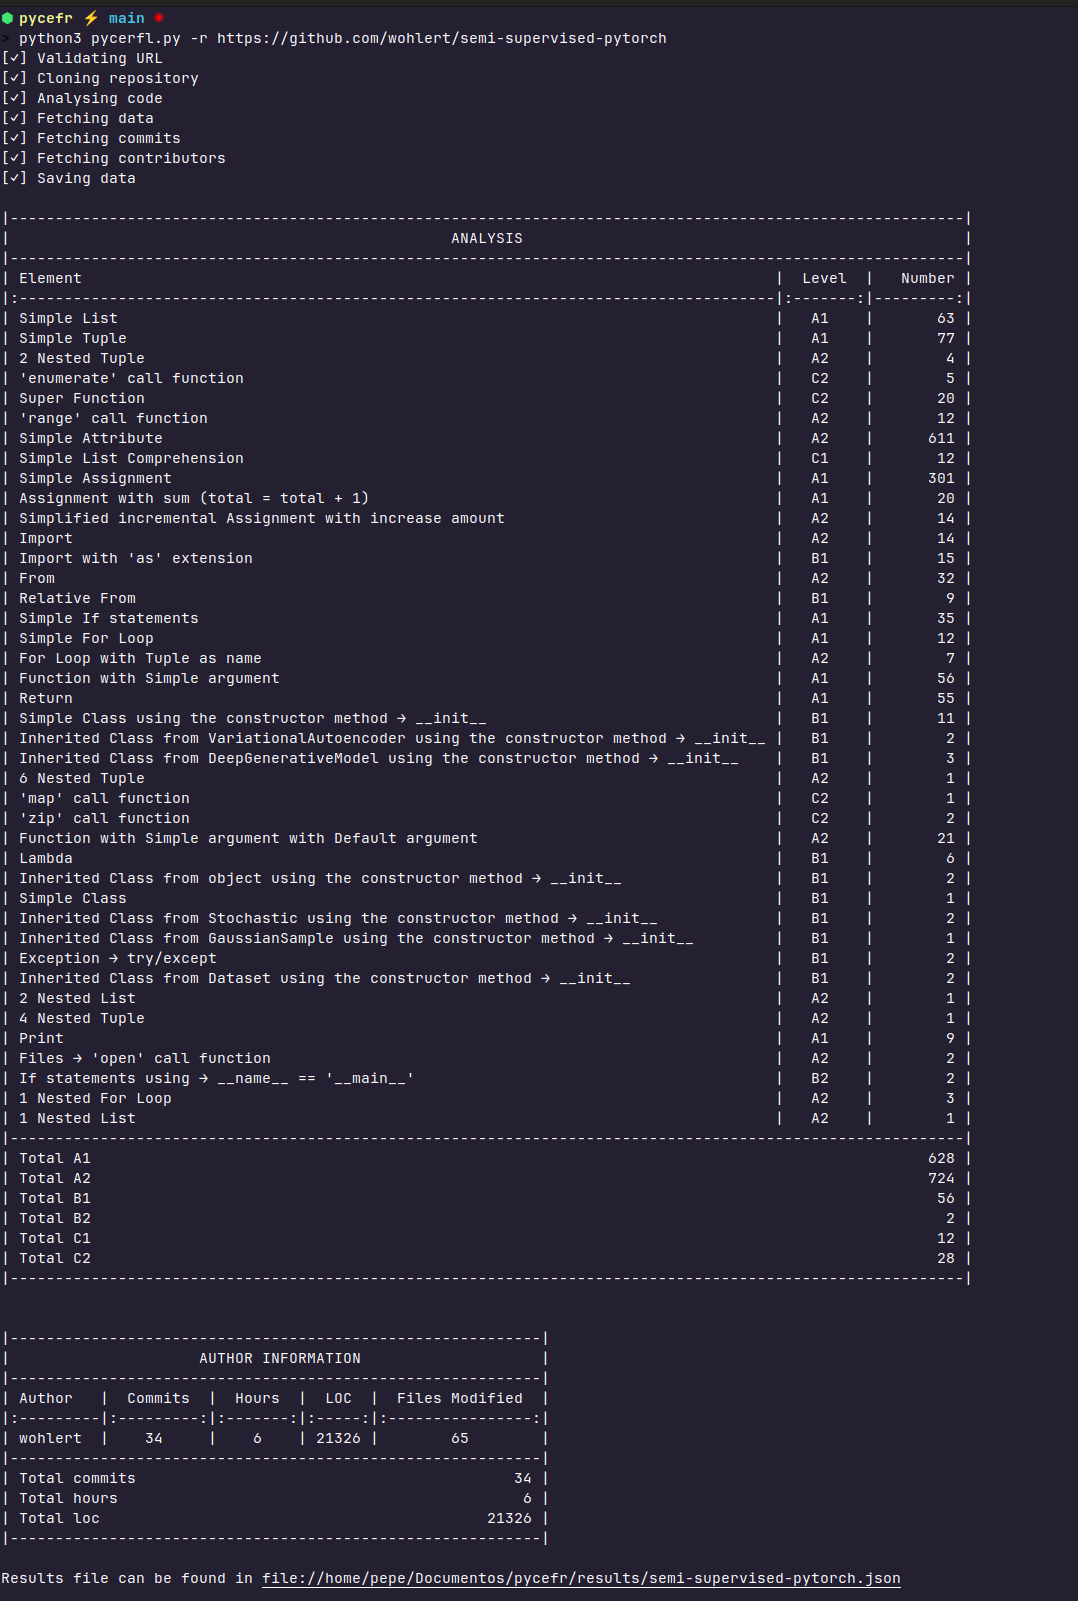
\includegraphics[height=\textheight, keepaspectratio]{img/results/backend_exe_r.png}
    \caption{Análisis completo de repositorio}
    \label{fig:analysis_repo}
\end{figure}


\subsection{Usuario (-u)}

Las opciones \texttt{-u <USER>} nos permiten analizar un repositorio dado un nombre de usuario de GitHub. 

En la figura 6.3 podemos ver este análisis. Hemos utilizado el mismo usuario de ejemplo, ``wohlert''. En este caso el programa nos lista los repositorios públicos de ``wohlert'' y nos pregunta cuál de ellos queremos analizar. Una vez seleccionado uno nos pide confirmar la acción, lo cual permite corregir la elección, y en caso de confirmar procede a realizar el análisis de dicho repositorio. Como en el caso anterior, se nos muestran mensajes indicando el estado del proceso y finalmente se imprimen los resultados por la consola.
\newpage
\begin{figure}[H]
    \centering
    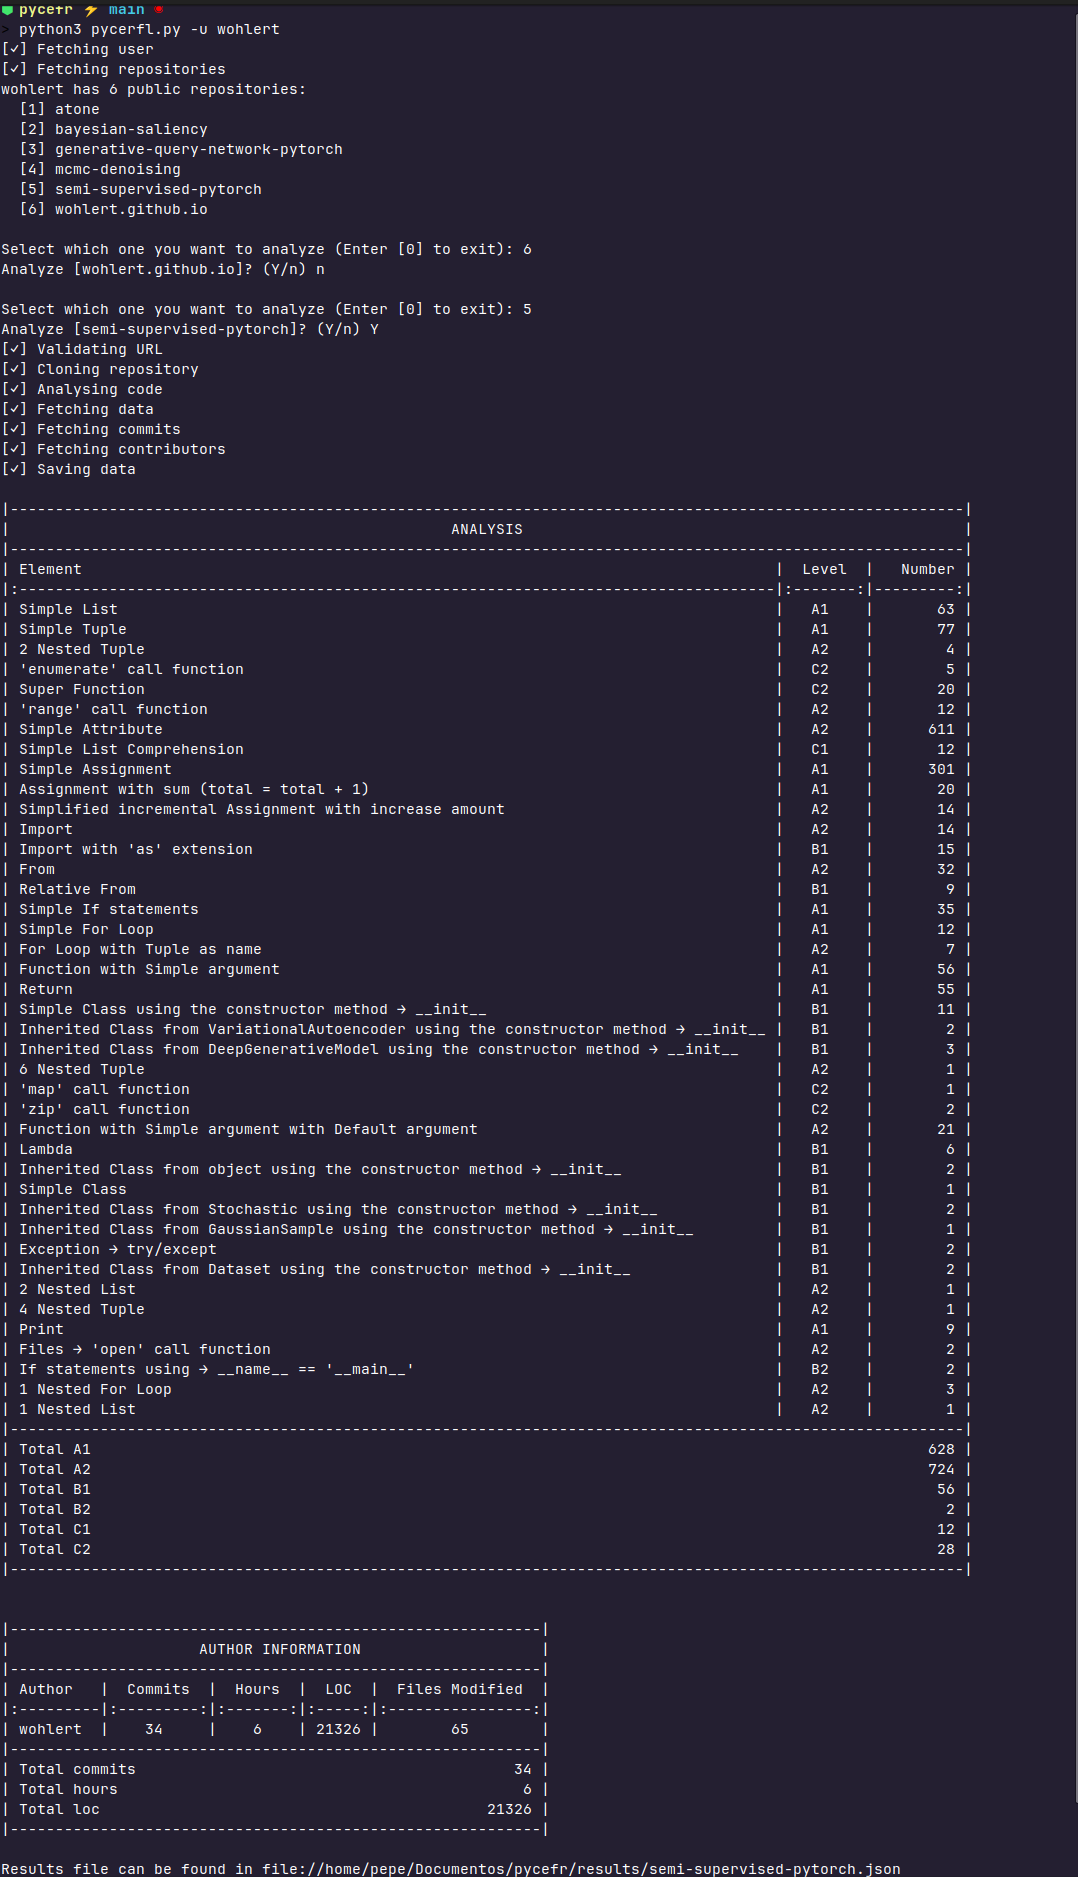
\includegraphics[height=\textheight, keepaspectratio]{img/results/backend_exe_u.png}
    \caption{Análisis de repositorio dado el usuario}
    \label{fig:analysis_user}
\end{figure}

\subsection{Directorio (-d)}

El caso \texttt{-d <DIR>} realiza un análisis de un repositorio local, dada la ruta del mismo. 

En este caso hemos clonado antes el repositorio que estamos empleando para las pruebas en la carpeta ``tmp/'', cuya finalidad es albergar archivos temporales cuya eliminación no altera la ejecución del programa.

La figura 6.4 nos muestra este proceso de clonado y el análisis del directorio. En este caso el programa nos dice que ha encontrado una configuración Git válida. Al tratarse de un directorio local es de esperar que no se incluya la información relativa al repositorio (puesto que no es un repositorio). Sin embargo, dado lo común que es trabajar con repositorios integrados en GitHub la aplicación comprueba si es el caso del directorio en cuestión. En caso de serlo, pregunta al usuario si prefiere analizar el repositorio remoto. Esto puede resultar ventajoso en caso de estar interesado en realizar un análisis con los cambios más recientes. 

Si el usuario responde de manera afirmativa se procede a realizar el análisis del repositorio (igual que si usáramos el argumento -r), ignorando los archivos locales. En caso negativo, se analiza el directorio indicado anteriormente. El archivo resultante se generará añadiendo el sufijo ``\_local'' al nombre del mismo. Esto da al usuario la oportunidad de realizar ambos análisis (local y del repositorio remoto) y no sobreescribir el archivo resultante (se toma el nombre del directorio o repositorio). Este comportamiento se puede activar o desactivar en el archivo de ajustes \texttt{settings.txt}, estableciendo en \textit{false} la opción \textit{addLocalSuffic}.

\newpage
\vspace{1em}
\begin{figure}[H]
    \centering
    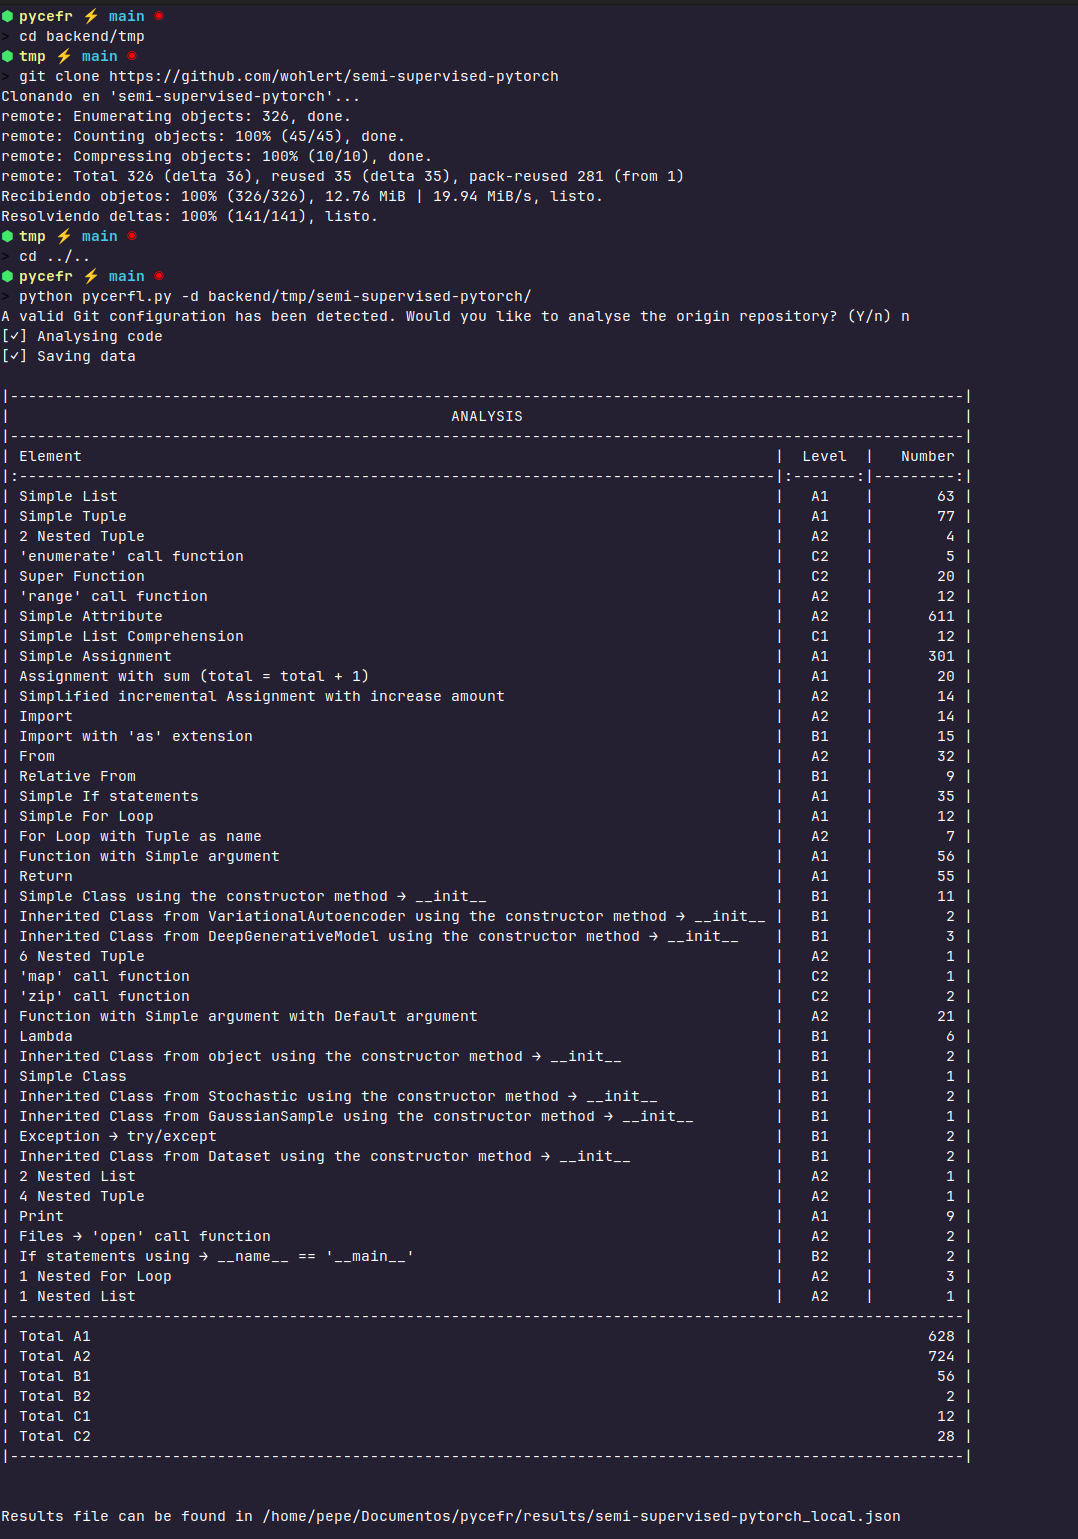
\includegraphics[height=17cm, keepaspectratio]{img/results/backend_exe_d.png}
    \caption{Análisis de directorio local}
    \label{fig:analysis_dir}
\end{figure}

\subsection{List (-l)}

La opción \texttt{-l} permite al usuario obtener el listado de los resultados existentes. Se nombran los archivos creados como consecuencia de los análisis realizados.

La figura 6.5 nos muestra este proceso, simple pero esencial para el uso del siguiente y último argumento disponible.

\begin{figure}
    \centering
    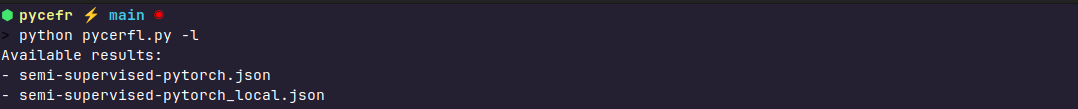
\includegraphics[width=\textwidth, keepaspectratio]{img/results/backend_exe_l.png}
    \caption{Listado de archivos de resultados}
    \label{fig:analysis_list}
\end{figure}

\subsection{Consola (-c)}

La última de las opciones disponibles, \texttt{-c <CONSOLE>} permite mostrar por consola resultados ya existentes, con el fin de evitar que tener que realizar de nuevo el análisis completo.

Tal como se presenta en la figura 6.6 hemos probado este argumento utilizando el archivo de resultados generado al comprobar el análisis de directorio local. Se nos muestra exactamente el mismo contenido, indicando primero los elementos encontrados, junto con su nivel y el número de instancias de cada uno, y finalmente agrupa por nivel todos los elementos, lo cual puede dar una mejor idea del nivel del proyecto.

\begin{figure}
    \centering
    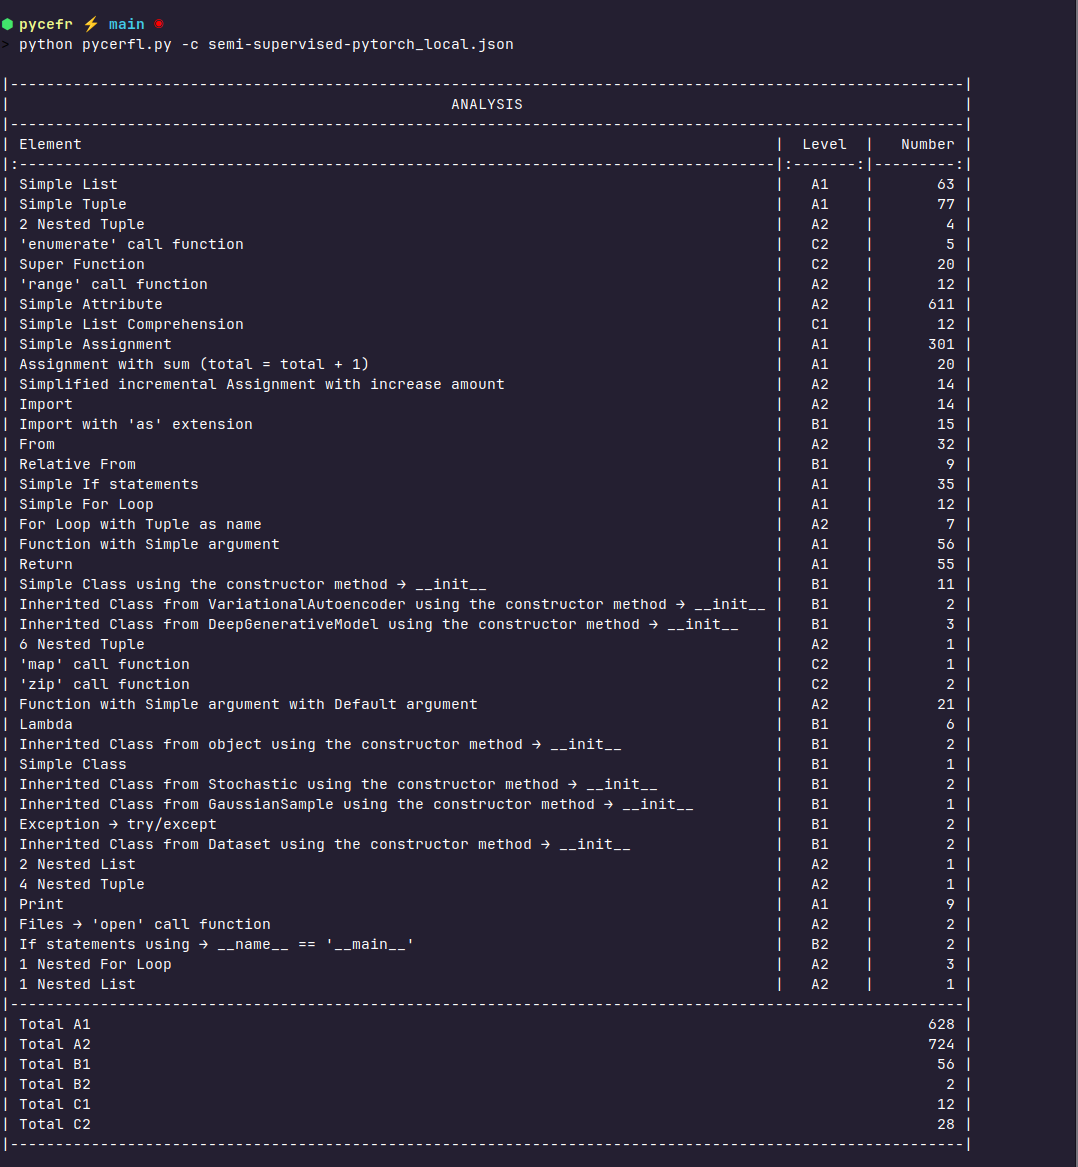
\includegraphics[width=\textwidth, keepaspectratio]{img/results/backend_exe_c.png}
    \caption{Mostrar resultados por consola}
    \label{fig:analysis_console}
\end{figure}
\clearpage

\subsection{Apuntes}
Es de especial relevancia mencionar el archivo de ajustes \texttt{settings.json}. Aunque ya hemos tratado algunas de las opciones disponibles falta mencionar la que probablemente sea la más importante de todas ellas.

A menudo los proyectos requieren de numerosos módulos y dependencias para su correcta ejecución. Éstos deben naturalmente estar instalados a la hora de ejecutar el proyecto, de lo contrario se producirían errores de ejecución. Por ejemplo, en este proyecto se está utilizando Python, y en este caso se requeren, entre otros, los módulos requests (utilizado para realizar solicitudes HTTP) o tabulate (para dar formato a los datos al mostrarlos por pantalla). Podríamos instalarlos en nuestra máquina, añadiéndolos a la versión de Python de ésta. Sin embargo, esto puede resultar problemático en caso de trabajar en varios proyectos que utilicen versiones distintas de un mismo módulo o dependencia.

La solución más ágil y común a este problema es la creación de un entorno virtual. Un entorno virtual es una herramienta que permite crear un espacio aislado en el que se pueden instalar y gestionar dependencias de proyectos sin interferir con otras instalaciones o proyectos en el mismo sistema. En nuestro caso hemos creado el entorno ``myenv'' para ello. Al crearse obtenemos un lienzo en blanco de Python al que añadir dependencias, lo cual hacemos mediante el uso del archivo \texttt{requirements.txt}. Esto nos sirve para el backend, escrito en Python; para el frontend, escrito en JavaScript, utilizamos una herramienta equivalente, llamada ``npm''.

En conclusión, estas carpetas de dependencias se almacenan dentro del proyecto y a menudo constan de un número muy elevado de archivos. Puesto que nuestro programa se dedica a analizar archivos, no nos conviene que se ``entretenga'' analizando estos numerosos (a veces incluso cientos), archivos. Es por ello en el archivo de ajustes hemos incluido una opción \textit{``ignoreFolders''}, en el que podemos incluir las carpetas que queremos excluir del análisis. En la figura 6.7 mostramos un ejemplo de uso, en el que aparecen las carpetas que hemos decidido ignorar para la realización de todas las pruebas.

\begin{figure}[H]
    \centering
    
\includegraphics[width=\textwidth, keepaspectratio]{img/results/ignore_folders.png}
    \caption{Ejemplo de uso de opción ``ignoreFolders''}
    \label{fig:ignore_folders}
\end{figure}

\section{Frontend}

Una vez visto el proceso para la creación del análisis podemos mostrar su visualización via web. Para ello nos posicionamos en la carpeta \texttt{frontend/} y levantamos el servidor ejecutando:

\begin{verbatim}
    node server.js
\end{verbatim}

\begin{figure}[H]
    \centering
    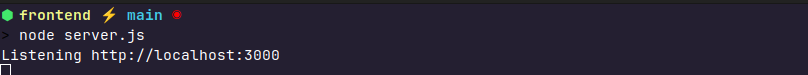
\includegraphics[width=\textwidth, keepaspectratio]{img/results/frontend_exe_console.png}
    \caption{Inicialización de servidor}
    \label{fig:frontend_console}
\end{figure}

Como se puede apreciar en la figura 6.8, el servidor nos indicará que está preparado para recibir solicitudes, añadiendo la dirección y el puerto por el que espera solicitudes. Por defecto se inicializará en el puerto 3000. Si vamos a esa dirección encontramos la página principal, la cual nos muestra un resumen de los análisis realizados.

\newpage
\vspace{1em}
\begin{figure}[H]
    \centering
    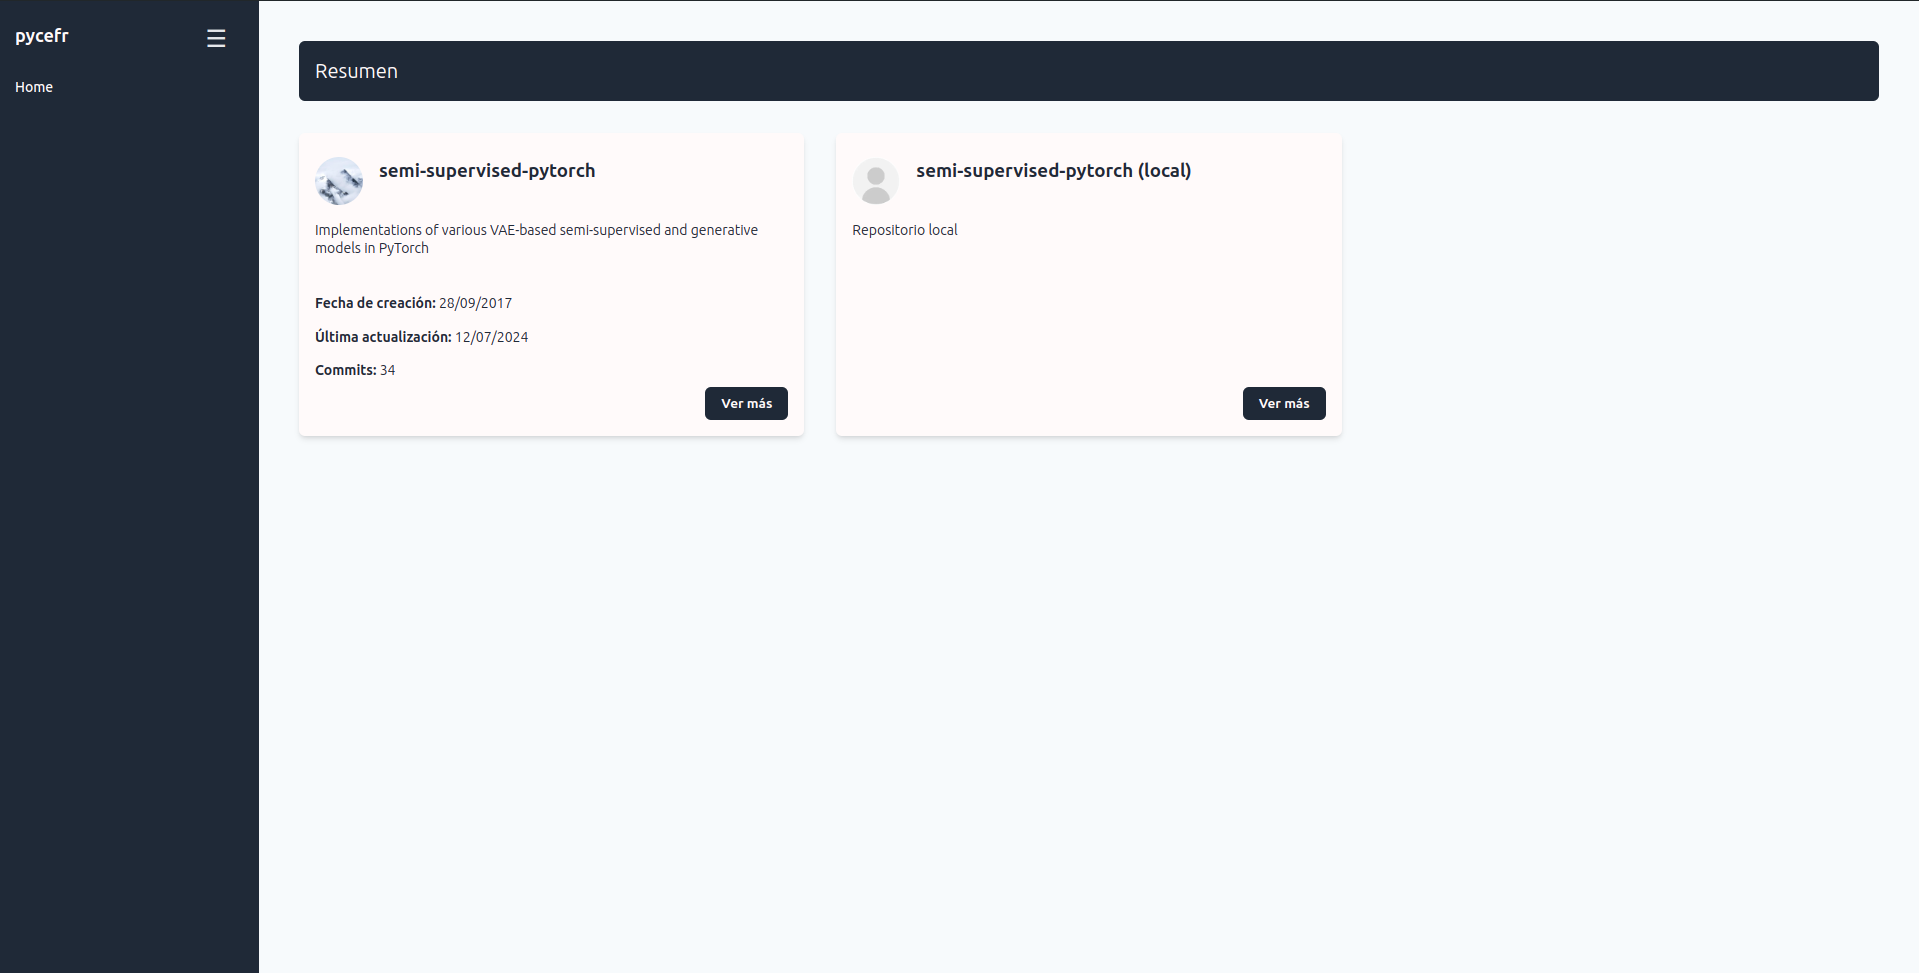
\includegraphics[width=\textwidth, keepaspectratio]{img/results/frontend_exe_home.png}
    \caption{Vista web: Home}
    \label{fig:frontend_home}
\end{figure}

Como se aprecia en la figura 6.9, en este caso se nos muestran dos resultados en la página principal, referentes a los dos análisis que hemos realizado. Aquí no podemos ver más que un breve resumen, para dar al usuario una pequeña idea del repositorio o directorio analizado. En caso de tratarse de un repositorio este resumen mostrará algunos datos relevantes sobre el mismo.

Al hacer click en el botón ``Ver más'' nos dirigimos a la página del propio análisis (ver figura 6.10). En este caso seleccionaremos el primero de ellos.

Diferenciamos en esta página dos bloques:

\begin{itemize}
    \item \textbf{Información general: } Como su propio nombre indica muestra información general del proyecto. Entre estos datos se encuentran el nombre del proyecto, su fecha de creación, el número de commits realizados, una estimación del número de horas empleadas en el proyecto y el número total de archivos y líneas modificados en la historia del proyecto.

    \item \textbf{Propiedades: } En esta tabla vemos finalmente el resultado del análisis. Dado el tipo de información he encontrado más conveniente representarlo en formato tabla. Para mejorar la experiencia del usuario, se ha añadido la capacidad de ordenar la tabla por cada columna, en orden ascendente o descendente.
\end{itemize}

Conviene mencionar que en el caso de seleccionar un directorio local no se muestra el primer bloque, de \textbf{información general}, puesto que no hay manera de mostrar, entre otros, el tiempo empleado en su edición o el número de archivos editados. Es por ello que he considerado mejor opción excluirlo antes que dedicar únicamente este bloque a mostrar el nombre del proyecto. Dicho esto, en línea con la política general del proyecto, se han creado estructuras y páginas de estilos pensando ya en futuros cambios o ampliaciones, en caso de querer mostrar más datos o incluso más bloques.

Por último, en todas las páginas (incluida la home) encontramos en la parte izquierda un menu para navegar por la web. Este menú se puede ocultar o mostrar haciendo click en el botón ``burguer'' en la esquina superior derecha, y de momento tiene un único enlace navegable para redirigirse a la home. Dada la funcionalidad actual del proyecto no he visto necesario añadir más opciones, pero me parece conveniente dejar hecho el propio menú, de modo que de ser necesario simplemente haya que añadir enlaces sin preocuparse del comportamiento del menú.

\vspace{1em}
\begin{figure}[ht]
    \centering
    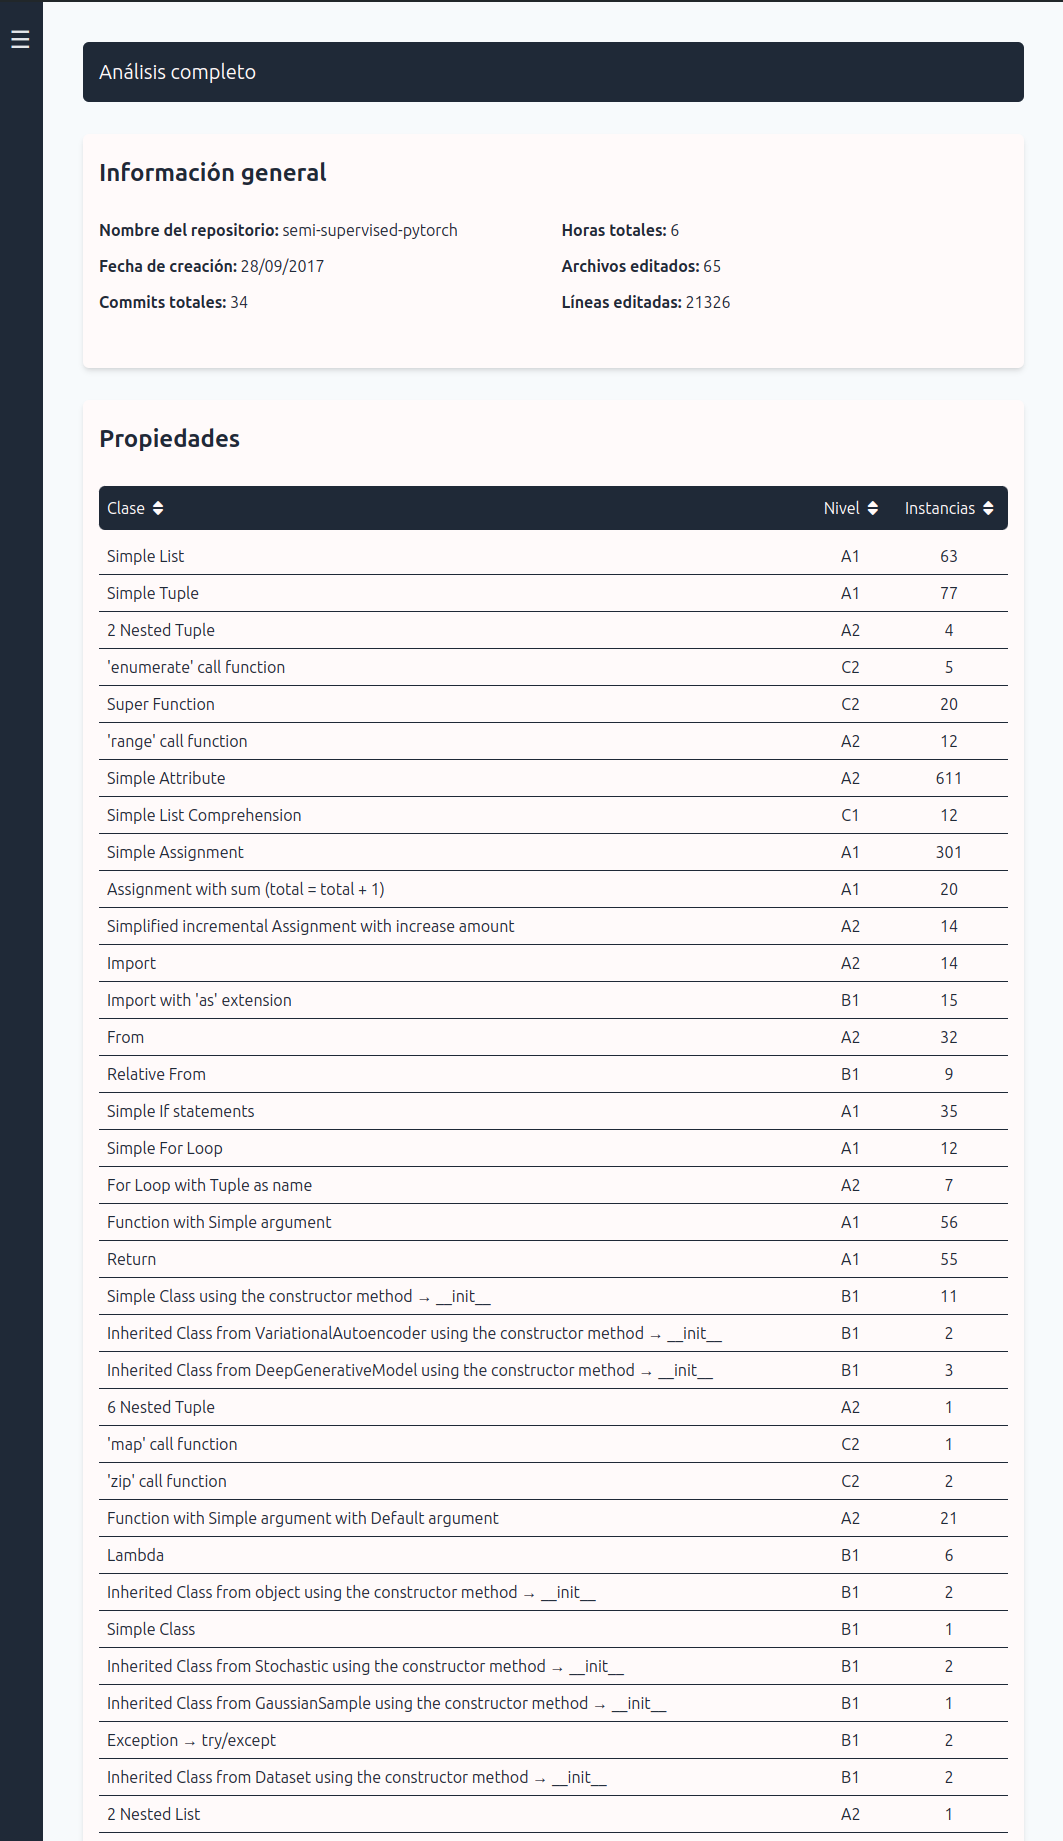
\includegraphics[height=\textheight, keepaspectratio]{img/results/frontend_exe_repo.png}
    \caption{Vista web: Repositorio}
    \label{fig:frontend_home}
\end{figure}

%%%%%%%%%%%%%%%%%%%%%%%%%%%%%%%%%%%%%%%%%%%%%%%%%%%%%%%%%%%%%%%%%%%%%%%%%%%%%%%%
%%%%%%%%%%%%%%%%%%%%%%%%%%%%%%%%%%%%%%%%%%%%%%%%%%%%%%%%%%%%%%%%%%%%%%%%%%%%%%%%
% CONCLUSIONES %
%%%%%%%%%%%%%%%%%%%%%%%%%%%%%%%%%%%%%%%%%%%%%%%%%%%%%%%%%%%%%%%%%%%%%%%%%%%%%%%%

\cleardoublepage
\chapter{Conclusiones}
\label{chap:conclusiones}


\section{Consecución de objetivos}
\label{sec:consecucion-objetivos}

Como hemos visto a lo largo de la sección de resultados se han cumplido la mayoría de las tareas propuestas inicialmente. 

\subsection{Mejora del código existente}

La mejora del código existente forma parte de casi todos los objetivos planteados. Sin embargo, considero que conviene mencionarlo como uno independiente para destacar el trabajo de refractorización del código en aras de simplificar su comprensión y edición. La abundante documentación añadida sirve el mismo propósito: facilitar la futura edición del proyecto.

\subsection{Implementación de funcionalidad ``plug-and-play''}

Personalmente éste era uno de los objetivos que primero me plantée y que consideraba prioritario. Me parecía de vital importancia dotar al usuario de la capacidad de ejecutar el programa nada más descargarlo. La inclusión de los archivos 'requisitos.txt' y 'package.json' para gestionar las dependencias del backend y del frontend, respectivamente, permiten a al usuario instalar en un par de segundos todo lo necesario. Esto junto con el cambio de rutas estáticas a rutas relativas en función del entorno de ejecución dan por cumplido este objetivo.

\subsection{Mejora de la visualización de los resultados en formato JSON}

Originalmente se generaban múltiples archivos que contenían a menudo la misma información pero de maneras distintas. Sin tener en cuenta todavía el uso de varios formatos, esto provocaba que incluso tras generar archivos de resultados había que crear nuevos archivos 'definitivos' de nuevo a partir de éstos. Se ha reducido a un solo archivo por análisis, facilitando al usuario el manejo de la información.

\subsection{Desarrollo de interfaz web}

El objetivo principal del proyecto era dotar al usuario de una mejor interfaz web para visualizar los datos. La original, aunque ténicamente funcional, era incómodo de usar para los estándares de hoy en día.

La implementación de una interfaz web navegable de manera cómoda y con la capacidad de ser expandida en el futuro, pues se ha diseñado de tal modo que esto resulte una tarea poco complicada, da por cumplido este objetivo.

\subsection{Implementar visualización de resultados por consola}

Además de la visualización web un objetivo importante era otorgar al usuario la capacidad de comprobar los resultados por consola, más rápido y ágil que la solución web. Se ha añadido esta vista en formato tabla, la cual considero más que intuitiva teniendo en cuenta el formato de información que estamos tratanto, y se ha incluido en un archivo de ajustes la capacidad de activar o desactivar el mostrado automático de los datos tras finalizar el análisis. Del mismo modo, el usuario puede ejecutar el programa de tal manera que en lugar de realizar el análisis simplemente imprima por la consola en el mismo formato resultados ya existentes. 

\subsection{Añadido de registros durante el proceso de análisis}

Aunque en el proyecto original había comentarios que explicaban qué tarea de estaba realizando, considero que los nuevos dan a entender al usuario de mejor manera qué está pasando en todo momento. Sin embargo, probablemente la mayor mejora se dé en los mensajes de error, antes ausentes, que ahora permiten al usuario saber qué está fallando exactamente, indicando incluso en caso de que el usuario pueda solventarlo la manera de hacerlo.

\subsection{Reestructuración de la arquitectura del código}

Al abordar el proyecto por primera vez el principal problema que tuve fue entender qué realizaba o cómo funcionaba exactamente. Ya no sólo por los problemas de ejecución iniciales, los cuales de acabaron resolviendo en un tiempo razonable, sino por la propia estructura del proyecto. Éste, debido a la relativa pequeña cantidad de archivos que contenía, no constaba de una estructura práctica ni mucho menos escalable.

Se han agrupado los archivos en carpetas que contienen lógica relacionada, facilitando así la organización y el acceso a los componentes del proyecto, intentando seguir los estándares modernos.

\subsection{Ampliación del análisis con información adicional}

Desde un inicio se ha pretendido expandir el análisis de dos maneras. La primera de ellas, incluyendo la información relativa a GitHub, esto es, información de los usuarios involucrados, del propio repositorio... La segunda parte consistía en rehacer el proceso completo de análisis, de modo que los elementos presentes en el código se contasen de una manera diferente para facilitar, de nuevo, su futura edición o personalización (se consideró otorgar al usuario la capacidad de activar y desactivar los elementos del código que analizar). Mientras que la primera tarea se cumplió sin mayor problema, al abordar este rediseño del análisis de archivos, me di cuenta de que era necesario reconstruir el proceso casi desde los cimientos. Tras reevaluar la magnitud de esta tarea consideré que el esfuerzo no justificaba la teórica diferencia de resultados, lo que llevó a replantear la viabilidad de este enfoque, finalmente optando por desecharlo. Dicho esto, se han realizado mejoras en los textos de los resultados.

\section{Aplicación de lo aprendido}
\label{sec:aplicacion}

La realización de este proyecto no habría sido posible de no ser por los conocimientos adquiridos en múltiples asignaturas del Grado de en Ingeniería en Tecnologías de la Telecomunicación. Al tratarse de un proyecto esencialmente de programación, no es de sorprender que las asignaturas que considere más me han aportado sean:

\begin{itemize}
    \item \textbf{Fundamentos de la programación: } La piedra angular de todo este proyecto. El conocimiento adquirido en esta asignatura, básico mas fundamental, es el que me ha permitido comenzar mi evolución como programador, sin la que no habría sido posible esta tarea.

    \item \textbf{Servicios y Aplicaciones Telemáticas: } Está asignatura me proporcionó por un lado el conocimiento de Python necesario para llevar a cabo este proyecto. Además, la elaboración de un gran proyecto en esta asignatura me hizo aprender a compaginar distintos lenguajes de programación en un mismo trabajo. Aunque no fuese un requisito indispensable de esta asignatura, fue ésta la que me impulsó a aprender en profundidad HTML y CSS, lenguajes que a día de hoy uso de manera extensa en el entorno laboral.

    \item \textbf{Desarrollo de Aplicaciones Telemáticas: } La asignatura que sin lugar a dudas considero que más me ha aportado en toda la carrera. Me permitió aprender JavaScript, uno de los lenguajes más utilizados a nivel mundial, a un ritmo personalizado, lo cual agradecí enormemente. Gracias a esta asignatura, junto con las anteriormente mencionadas, pude realizar mis labores más tarde en las prácticas externas.

    \item \textbf{Prácticas Externas: } El conocimiento adquirido en las asignaturas ya mencionadas me permitió tomar parte en una empresa como desarrollador web. Dejando a un lado el conocimiento adquirido en relación a los lenguajes empleados aquí aprendí sobre todo qué es el trabajo a nivel empresa, con todo lo que eso conlleva.
    
\end{itemize}


\section{Lecciones aprendidas}
\label{sec:lecciones_aprendidas}

Las lecciones aprendidas tras la elaboración de este proyecto son:

\begin{itemize}
    \item Consolidación de conocimientos del framework Express.js, visto en la asignatura 'Desarrollo de Aplicaciones Telemáticas' y Node.js.
    \item Uso de la herramienta Postman para la realización de pruebas con API.
    \item Patrones de diseño y sintaxis de Python con los que no estaba familiarizado.
    \item Estándares de desarrollo web modernos.
\end{itemize}

\section{Trabajos futuros}
\label{sec:trabajos_futuros}

En el futuro podrían implementarse las siguientes funcionalidades:

\begin{itemize}
    \item Edición del sistema de análisis. Permitir al usuario poder añadir o quitar elementos del análisis, así como poder estipular por sí mismo el nivel que cada elemento analizado.
    \item Funcionalidad completa del proyecto desde la página web, sin depender de ejecutar el proyecto anteriormente desde la consola. Es decir, poder realizar el análisis directamente desde la web.
    \item Interacciones entre varios archivos de resultados (comparar archivos, unirlos...). 
\end{itemize}


%%%%%%%%%%%%%%%%%%%%%%%%%%%%%%%%%%%%%%%%%%%%%%%%%%%%%%%%%%%%%%%%%%%%%%%%%%%%%%%%
%%%%%%%%%%%%%%%%%%%%%%%%%%%%%%%%%%%%%%%%%%%%%%%%%%%%%%%%%%%%%%%%%%%%%%%%%%%%%%%%
% APÉNDICE(S) %
%%%%%%%%%%%%%%%%%%%%%%%%%%%%%%%%%%%%%%%%%%%%%%%%%%%%%%%%%%%%%%%%%%%%%%%%%%%%%%%%

\cleardoublepage
\appendix
\chapter{Manual de usuario}
\label{app:manual}

\textbf{pycefr} es una herramienta diseñada para evaluar el nivel de código Python 3 utilizando como inspiración el Marco Común Europeo de Referencia para las Lenguas (CERFL). Permite analizar repositorios de GitHub y directorios locales para proporcionar información valiosa sobre el nivel del código.

\section{Requisitos Previos}
Antes de comenzar, asegúrate de tener instalado Python 3 y Node.js. Asegúrate también de tener los permisos adecuados para acceder a los directorios que deseas analizar.

Puedes instalar los módulos de Python necesarios utilizando el archivo \texttt{requirements.txt} ejecutando el siguiente comando:

\begin{verbatim}
pip install -r requirements.txt
\end{verbatim}

Además, para instalar los módulos de Node.js requeridos, navega a la carpeta \texttt{frontend/} y ejecuta:

\begin{verbatim}
npm install
\end{verbatim}

\section{Estructura del Proyecto}
El proyecto incluye los siguientes componentes principales:

\begin{itemize}
    \item \textbf{pycefr.py}: El ejecutable principal que realiza el análisis.
    \item \textbf{backend/}: Carpeta que contiene los archivos que realizan el análisis del código
    \item \textbf{frontend/}: Carpeta que contiene la interfaz de usuario basada en Node.js para visualizar los resultados.
    \item \textbf{results/}: Carpeta donde se almacenan los resultados del análisis.
\end{itemize}

Se incluyen también varios archivos secundarios, encargados de la configuración de la aplicación o de 
\begin{itemize}
    \item \textbf{settings.json}: Archivo de configuración para personalizar la herramienta.
    \item \textbf{pycefrl.postman\_collection.json}: Colección de Postman con las llamadas involucradas en el proyecto.
    \item \textbf{requirements.txt}: Archivo utilizado para instalar los módulos de Python necesarios.
\end{itemize}

\section{Cómo Usar pycefr}

\subsection{1. Análisis de un Repositorio de GitHub}
Para analizar un repositorio de GitHub, utiliza el siguiente comando:
\begin{verbatim}
python3 pycerfl.py -r <repo_url>
\end{verbatim}
Este comando realiza un análisis completo en un repositorio válido de GitHub.

\subsection{2. Análisis de un Usuario de GitHub}
Para obtener información sobre un usuario de GitHub y sus proyectos, usa:
\begin{verbatim}
python3 pycerfl.py -u <user_name>
\end{verbatim}
El sistema te preguntará cuál de los proyectos públicos del usuario deseas analizar.

\subsection{3. Análisis de un Directorio Local}
Para analizar un directorio local, ejecuta:
\begin{verbatim}
python3 pycerfl.py -d <dir_path>
\end{verbatim}
Este comando realizará un análisis completo en el directorio especificado.

\subsection{4. Listar Archivos de Resultados}
Para listar los archivos generados en la carpeta \texttt{results/}, puedes usar la opción:
\begin{verbatim}
python3 pycerfl.py -l
\end{verbatim}

\subsection{5. Visualizar resultados por consola}
Para visualizar un archivo de resultados por consola puedes usar la opción:
\begin{verbatim}
python3 pycerfl.py -c <results_file>
\end{verbatim}
\subsection{6. Visualización de Resultados via web}
Una vez completado el análisis, se generará un archivo JSON en la carpeta \texttt{results/}. Para visualizar estos resultados, puedes usar Node.js:
\begin{enumerate}
    \item Navega a la carpeta \texttt{frontend/} y ejecuta:
    \begin{verbatim}
    npm install
    \end{verbatim}
    \item Luego, ejecuta el servidor local:
    \begin{verbatim}
    node server.js
    \end{verbatim}
\end{enumerate}
Abre tu navegador y dirígete a \texttt{http://localhost:3000} para ver los resultados.

\subsection{Configuración de settings.json}
El archivo \texttt{settings.json} permite personalizar la configuración de la herramienta:
\vspace{1em}

\begin{tabular}{|l|p{10cm}|} % Ajusta el ancho de la columna según necesites
\hline
\textbf{Ajustes} & \textbf{Descripción} \\
\hline
\texttt{ignoreFolders} & Lista de carpetas que serán excluidas del análisis. \\
\texttt{API-KEY} & Clave API de GitHub para evitar el límite en las llamadas a la API. \\
\texttt{addLocalSuffix} & Si se establece en \texttt{true}, añade el sufijo \texttt{\_local} a los archivos de resultados. \\
\texttt{autoDisplayConsole} & Si se establece en \texttt{true}, muestra los resultados por consola tras finalizar el análisis. \\
\hline
\end{tabular}

\vspace{1em}
\subsubsection{Ejemplo de settings.json}
\begin{verbatim}
{
    ``ignoreFolders'': [
        "node_modules/",
        "myenv/",
        ".git/",
        "__pycache__/"
    ],
    "API-KEY": "customapikey1234",
    "addLocalSuffix": true
    "autoDisplayConsole": true
}
\end{verbatim}

\subsection{Importación de colección Postman}

En caso de querer probar las llamadas realizadas en el código tenemos la posibilidad de importar en Postman el archivo \texttt{pycerfl.postman\_collection.json} y ver todas las solicitudes con ejemplos de uso. Para ello abrimos Postman y en seleccionamos la opción ``Import'' en la parte superior. Esto nos abrirá el siguiente panel:

\begin{figure}[H]
    \centering
    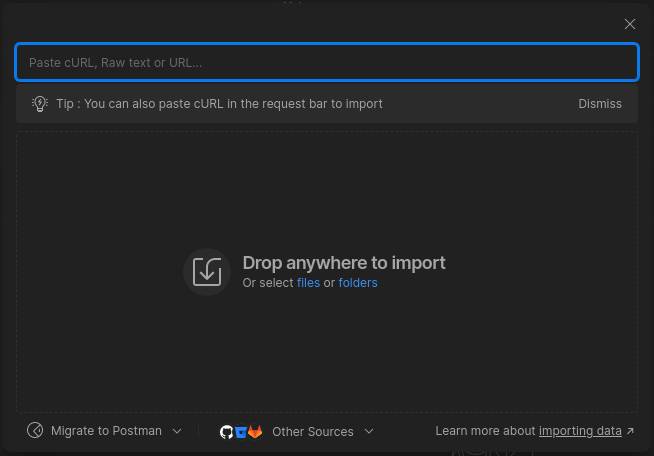
\includegraphics[width=\linewidth]{img/postman_import.png}
    \caption{Panel de importación en Postman}
    \label{fig:postman_import}
\end{figure}

Añadimos el archivo ya sea haciendo click o arrastrándolo directamente. Tras esto ya tendremos acceso a todas las llamadas involucradas en el proyecto.
%%%%%%%%%%%%%%%%%%%%%%%%%%%%%%%%%%%%%%%%%%%%%%%%%%%%%%%%%%%%%%%%%%%%%%%%%%%%%%%%
%%%%%%%%%%%%%%%%%%%%%%%%%%%%%%%%%%%%%%%%%%%%%%%%%%%%%%%%%%%%%%%%%%%%%%%%%%%%%%%%
% BIBLIOGRAFIA %
%%%%%%%%%%%%%%%%%%%%%%%%%%%%%%%%%%%%%%%%%%%%%%%%%%%%%%%%%%%%%%%%%%%%%%%%%%%%%%%%

\cleardoublepage

% Las siguientes dos instrucciones es todo lo que necesitas
% para incluir las citas en la memoria
\bibliographystyle{abbrv}
\bibliography{memoria}  % memoria.bib es el nombre del fichero que contiene
% las referencias bibliográficas. Abre ese fichero y mira el formato que tiene,
% que se conoce como BibTeX. Hay muchos sitios que exportan referencias en
% formato BibTeX. Prueba a buscar en http://scholar.google.com por referencias
% y verás que lo puedes hacer de manera sencilla.
% Más información: 
% http://texblog.org/2014/04/22/using-google-scholar-to-download-bibtex-citations/

\end{document}
